\chapter{SCI-HI System Development}\label{Ch:System}

\section{Overview} \label{Sec:sysover}
$''$Sonda Cosmologica de las Islas para la Deteccion de Hidrogeno Neutro$''$ (SCI-HI) is an experiment which seeks to measure the \cm global spectrum during the end of the Dark Ages and the Cosmic Dawn before reionization. As such, SCI-HI instrument was designed to meet several distinct contraints:

\begin{enumerate}
\item The design must be low cost (under \$10,000).

\item The design must be low power (under  200 Watts) so that it can be run with an independent power source separate from external supplies. 

\item The design must be simple and easy to deploy to remote locations. 

\item The design must be broad-band to cover the wide bandwidth of interest ($40-130$ MHz).

\item The design must include a system response that varies smoothly with frequency. 

\end{enumerate}

\begin{figure}[htb]
\begin{center}
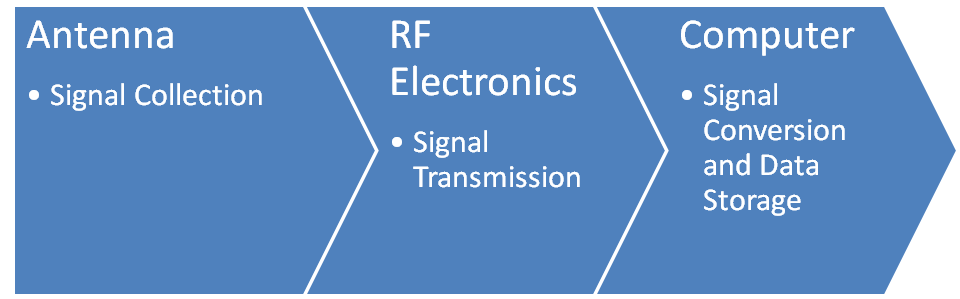
\includegraphics[width=0.9\linewidth]{SCIHI_system/figures/basic_block_diagram.png}
\caption{Basic Block Diagram of the SCI-HI instrument.}
\label{Fig:basic_block_diagram}
\end{center}
\end{figure}

In order to meet these constraints, the instrument design was broken down into three categories based upon their purpose in the overall design (see Figure \ref{Fig:basic_block_diagram}). These categories are an antenna for signal collection, radio frequency (RF) electronics for calibration and signal transmission, and a computer for signal processing and storage.

\section{Antenna}
When designing an instrument for radio astronomy, one of the big challenges is finding an antenna design that fits the particular needs of a given experiment. 

\subsection{Design Considerations}
For the SCI-HI experiment, the key properties for the antenna selection were the bandwidth and stability of the antenna beam pattern and impedance (S-parameters) over frequency. 

\textcolor{red}{Here I will add a brief discussion of antenna design including some of the key parameters for an antenna in general and why they are significant. }

\begin{figure}[htb]
\centering
\begin{minipage}[b]{0.45\textwidth}
\centering
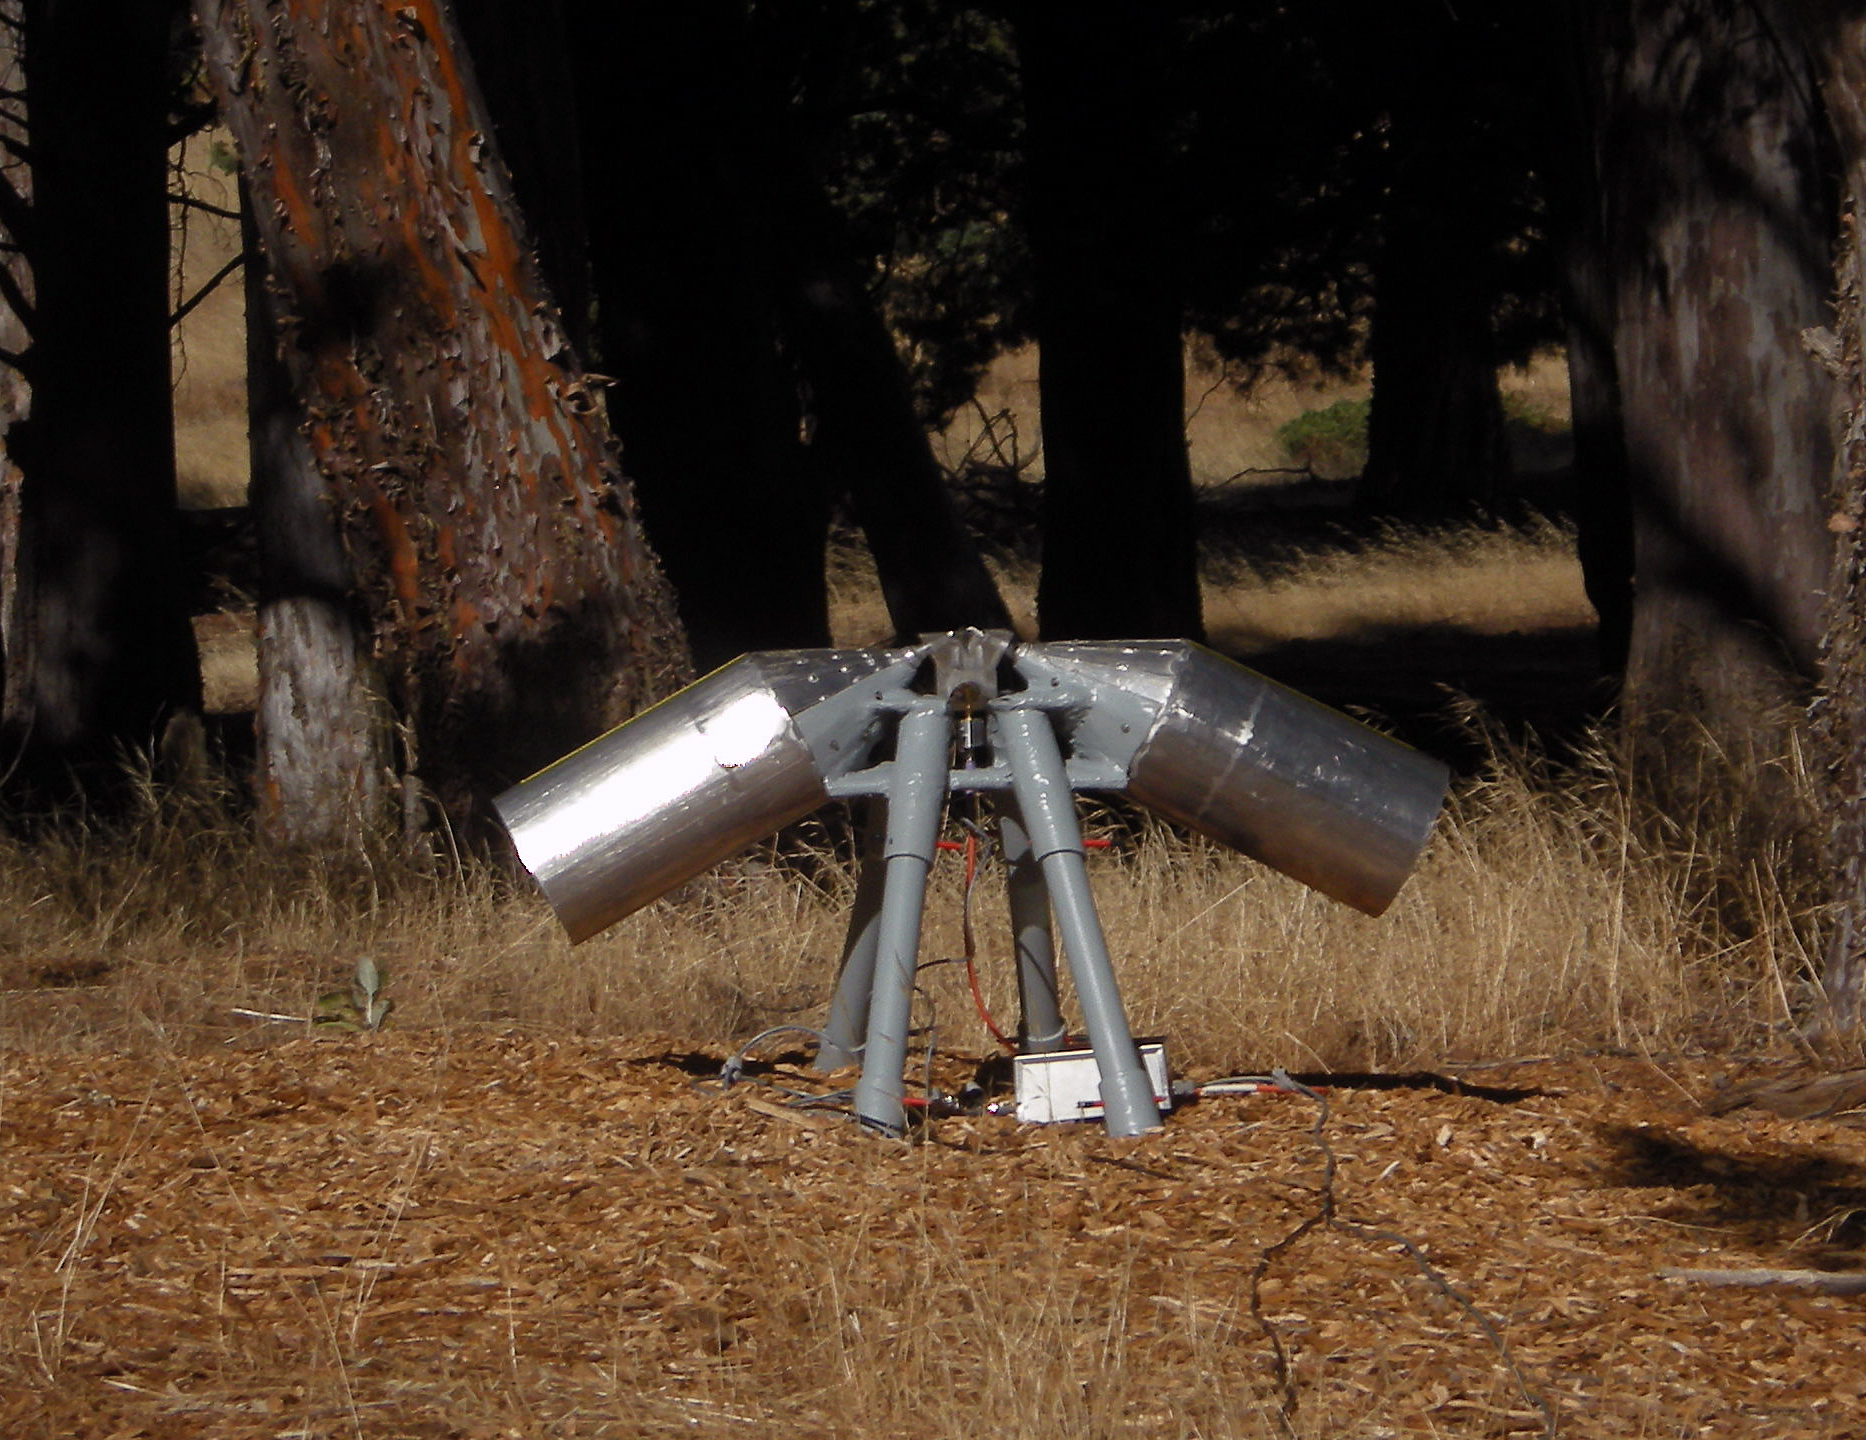
\includegraphics[width=0.95\linewidth]{SCIHI_system/figures/trombone_guad_small.jpg}
\caption{Trombone Antenna setup in its smallest (highest center frequency) configuration.}
\label{Fig:trombone_small}
\end{minipage}%
\begin{minipage}[b]{0.02\textwidth}
\hspace{1cm}
\end{minipage}%
\begin{minipage}[b]{0.51\textwidth}
\centering
\includegraphics[width=0.95\linewidth]{SCIHI_system/figures/trombone_pgh_zoom.jpg}
\caption{Trombone Antenna setup in its largest (lowest center frequency) configuration.}
\label{Fig:trombone_large}
\end{minipage}
\end{figure}

\subsection{First Stage Antenna}
Initially, we started with a simple $''$Trombone$''$ antenna. This design is a dipole with fat, angled elements over a ground plane (see Figures \ref{Fig:trombone_small} and \ref{Fig:trombone_large}). Changing the frequency range of the antenna simply required shifting the length of the dipole elements and their position above the ground plane. 

The design was based on the idea that features in the measured spectrum which were from the sky would stay at the same frequencies when the antenna was tuned. On the other hand, features in the measured spectrum from the antenna would shift. This shifting would allow us to distinguish real structure on the sky such as the \cm signal from structure due to the antenna. 

\begin{figure}[htb]
\centering
\begin{minipage}[b]{0.53\textwidth}
\centering
\includegraphics[width=0.95\linewidth]{SCIHI_system/figures/trombone_mount.jpg}
\caption{Mounting for the Trombone antenna, with lucite mount point and fiberglass support structure. }
\label{Fig:trombone_mount}
\end{minipage}%
\begin{minipage}[b]{0.02\textwidth}
\hspace{1cm}
\end{minipage}%
\begin{minipage}[b]{0.41\textwidth}
\centering
\includegraphics[width=0.95\linewidth]{SCIHI_system/figures/trombone_guad_adj.jpg}
\caption{Changing the Trombone antenna configuration from small to large.}
\label{Fig:trombone_adj}
\end{minipage}
\end{figure}

\subsubsection{Antenna Construction}
The trombone shapes were constructed out of welded aluminum with a lucite mounting block at the connection point of the two cones (see Figure \ref{Fig:trombone_mount}), The dipoles and mounting block were supported with a structure constructed out of fiberglass and PVC tubes. The entire system was placed above a ground plane composed of metal mesh (aka chicken wire) over a small ($\sim9 m^2$) area and long radial extensions ($\sim10 m$) extending out from the center like a spider web. 

Tuning the trombone length was accomplished with an external tube that slid over the main dipole elements (see Figure \ref{Fig:trombone_adj}), while adjustment of the height of the trombone was done using the support legs (PVC pipes with variable heights).

\begin{figure}[htb]
\centering
\begin{minipage}[b]{0.48\textwidth}
\centering
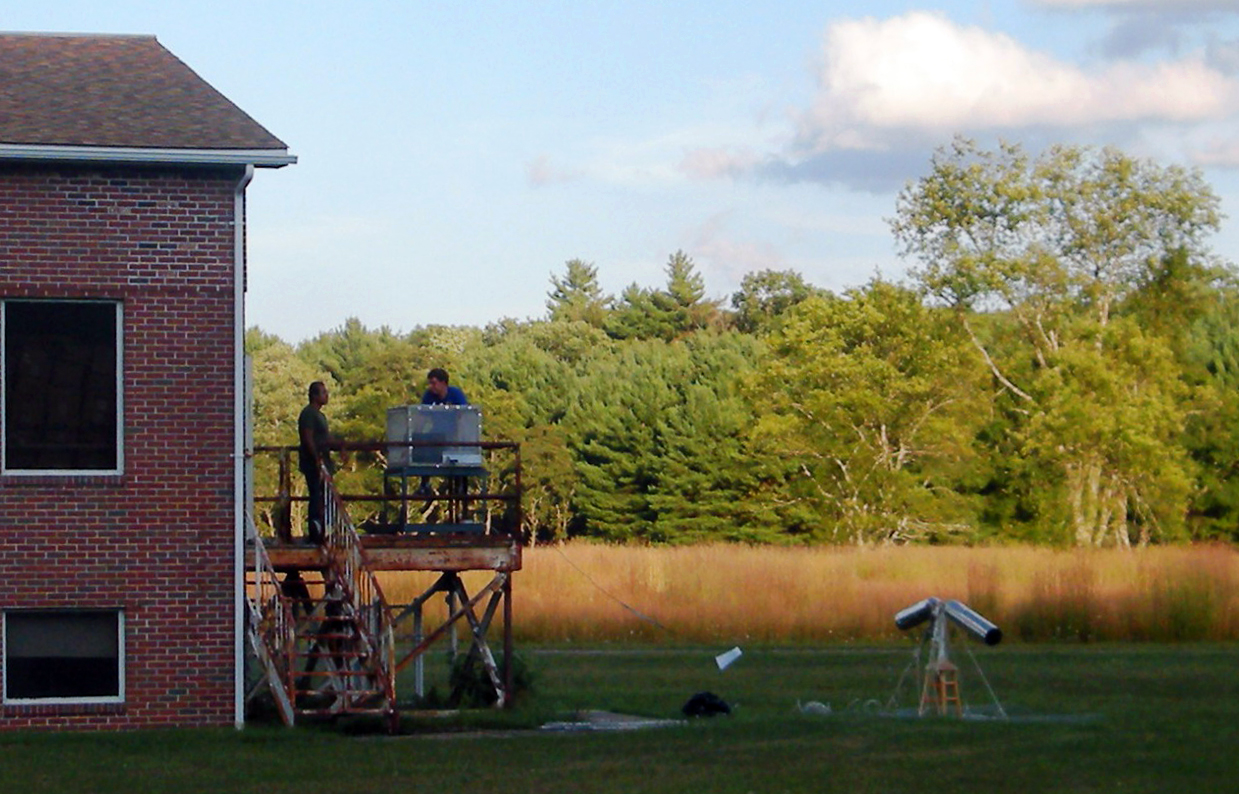
\includegraphics[width=0.95\linewidth]{SCIHI_system/figures/trombone_gbt.jpg}
\caption{SCI-HI setup with trombone antenna on site at Green Bank in August 2011.}
\label{Fig:trombone_gbt}
\end{minipage}%
\begin{minipage}[b]{0.02\textwidth}
\hspace{1cm}
\end{minipage}%
\begin{minipage}[b]{0.46\textwidth}
\centering
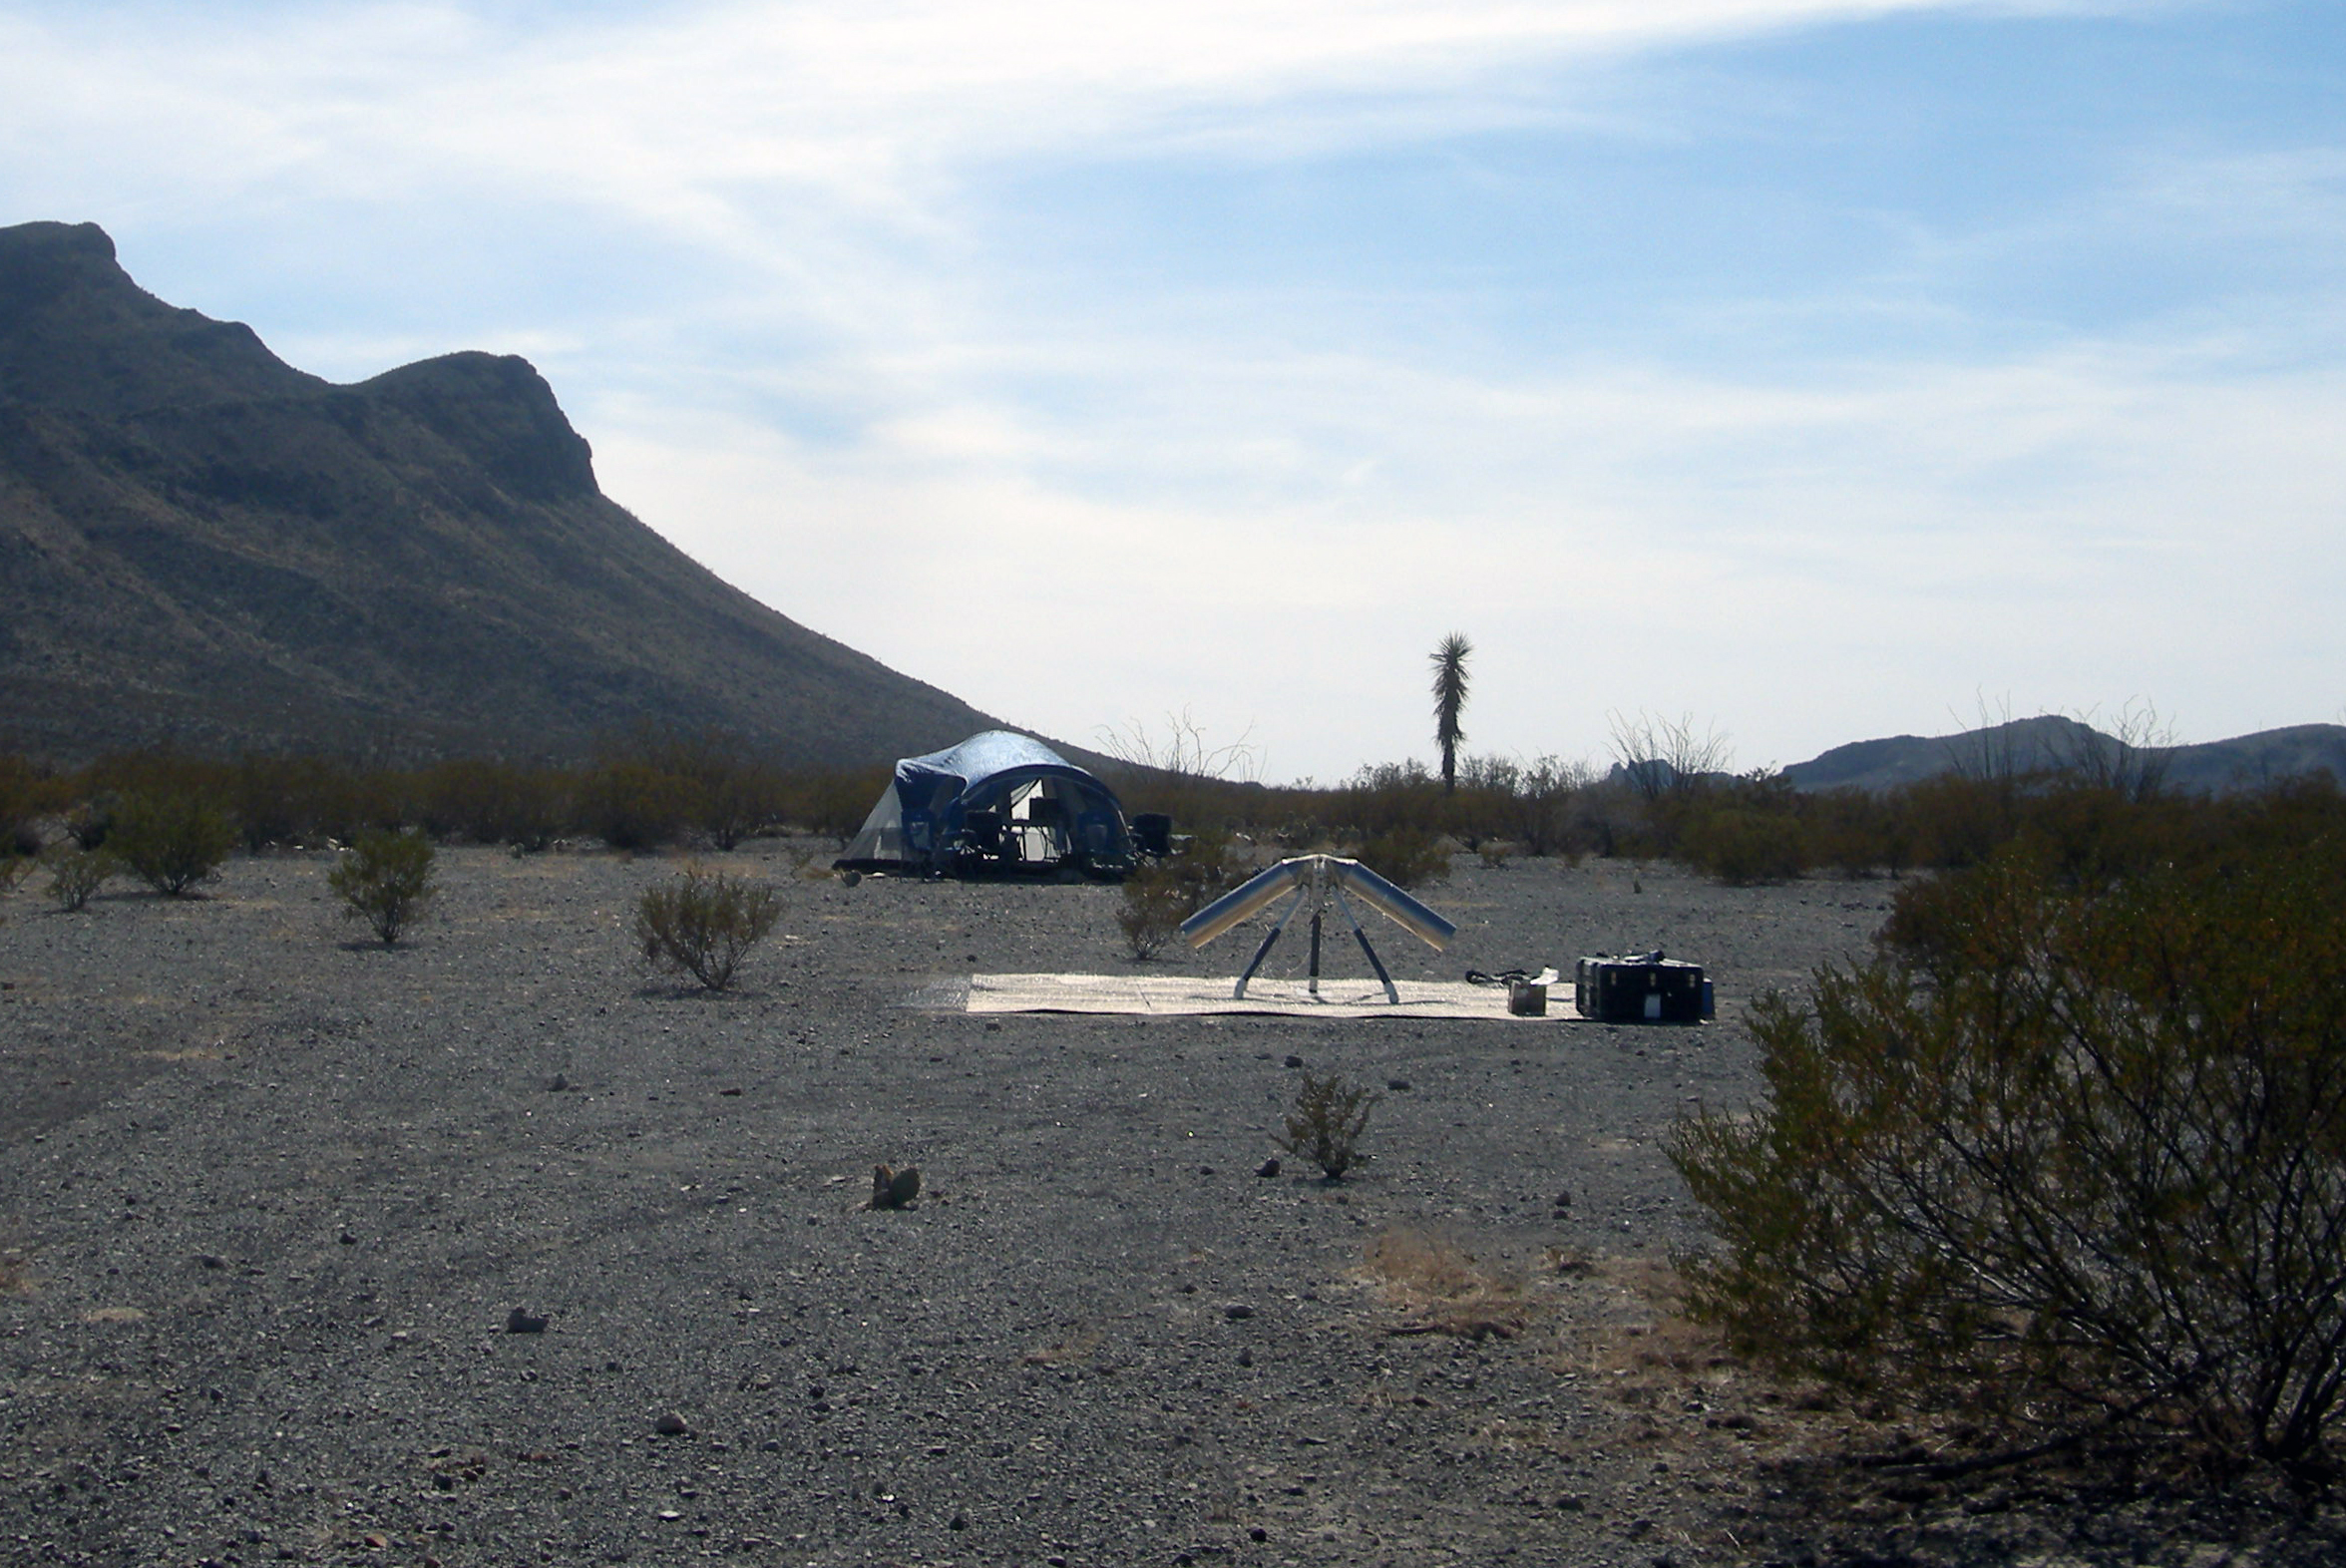
\includegraphics[width=0.95\linewidth]{SCIHI_system/figures/trombone_sys_ZdS.jpg}
\caption{SCI-HI setup with trombone antenna on site at the Zona del Silencio in January 2012.}
\label{Fig:trombone_zds}
\end{minipage}
\end{figure}

\begin{figure}[htb]
\centering
\begin{minipage}[b]{0.52\textwidth}
\centering
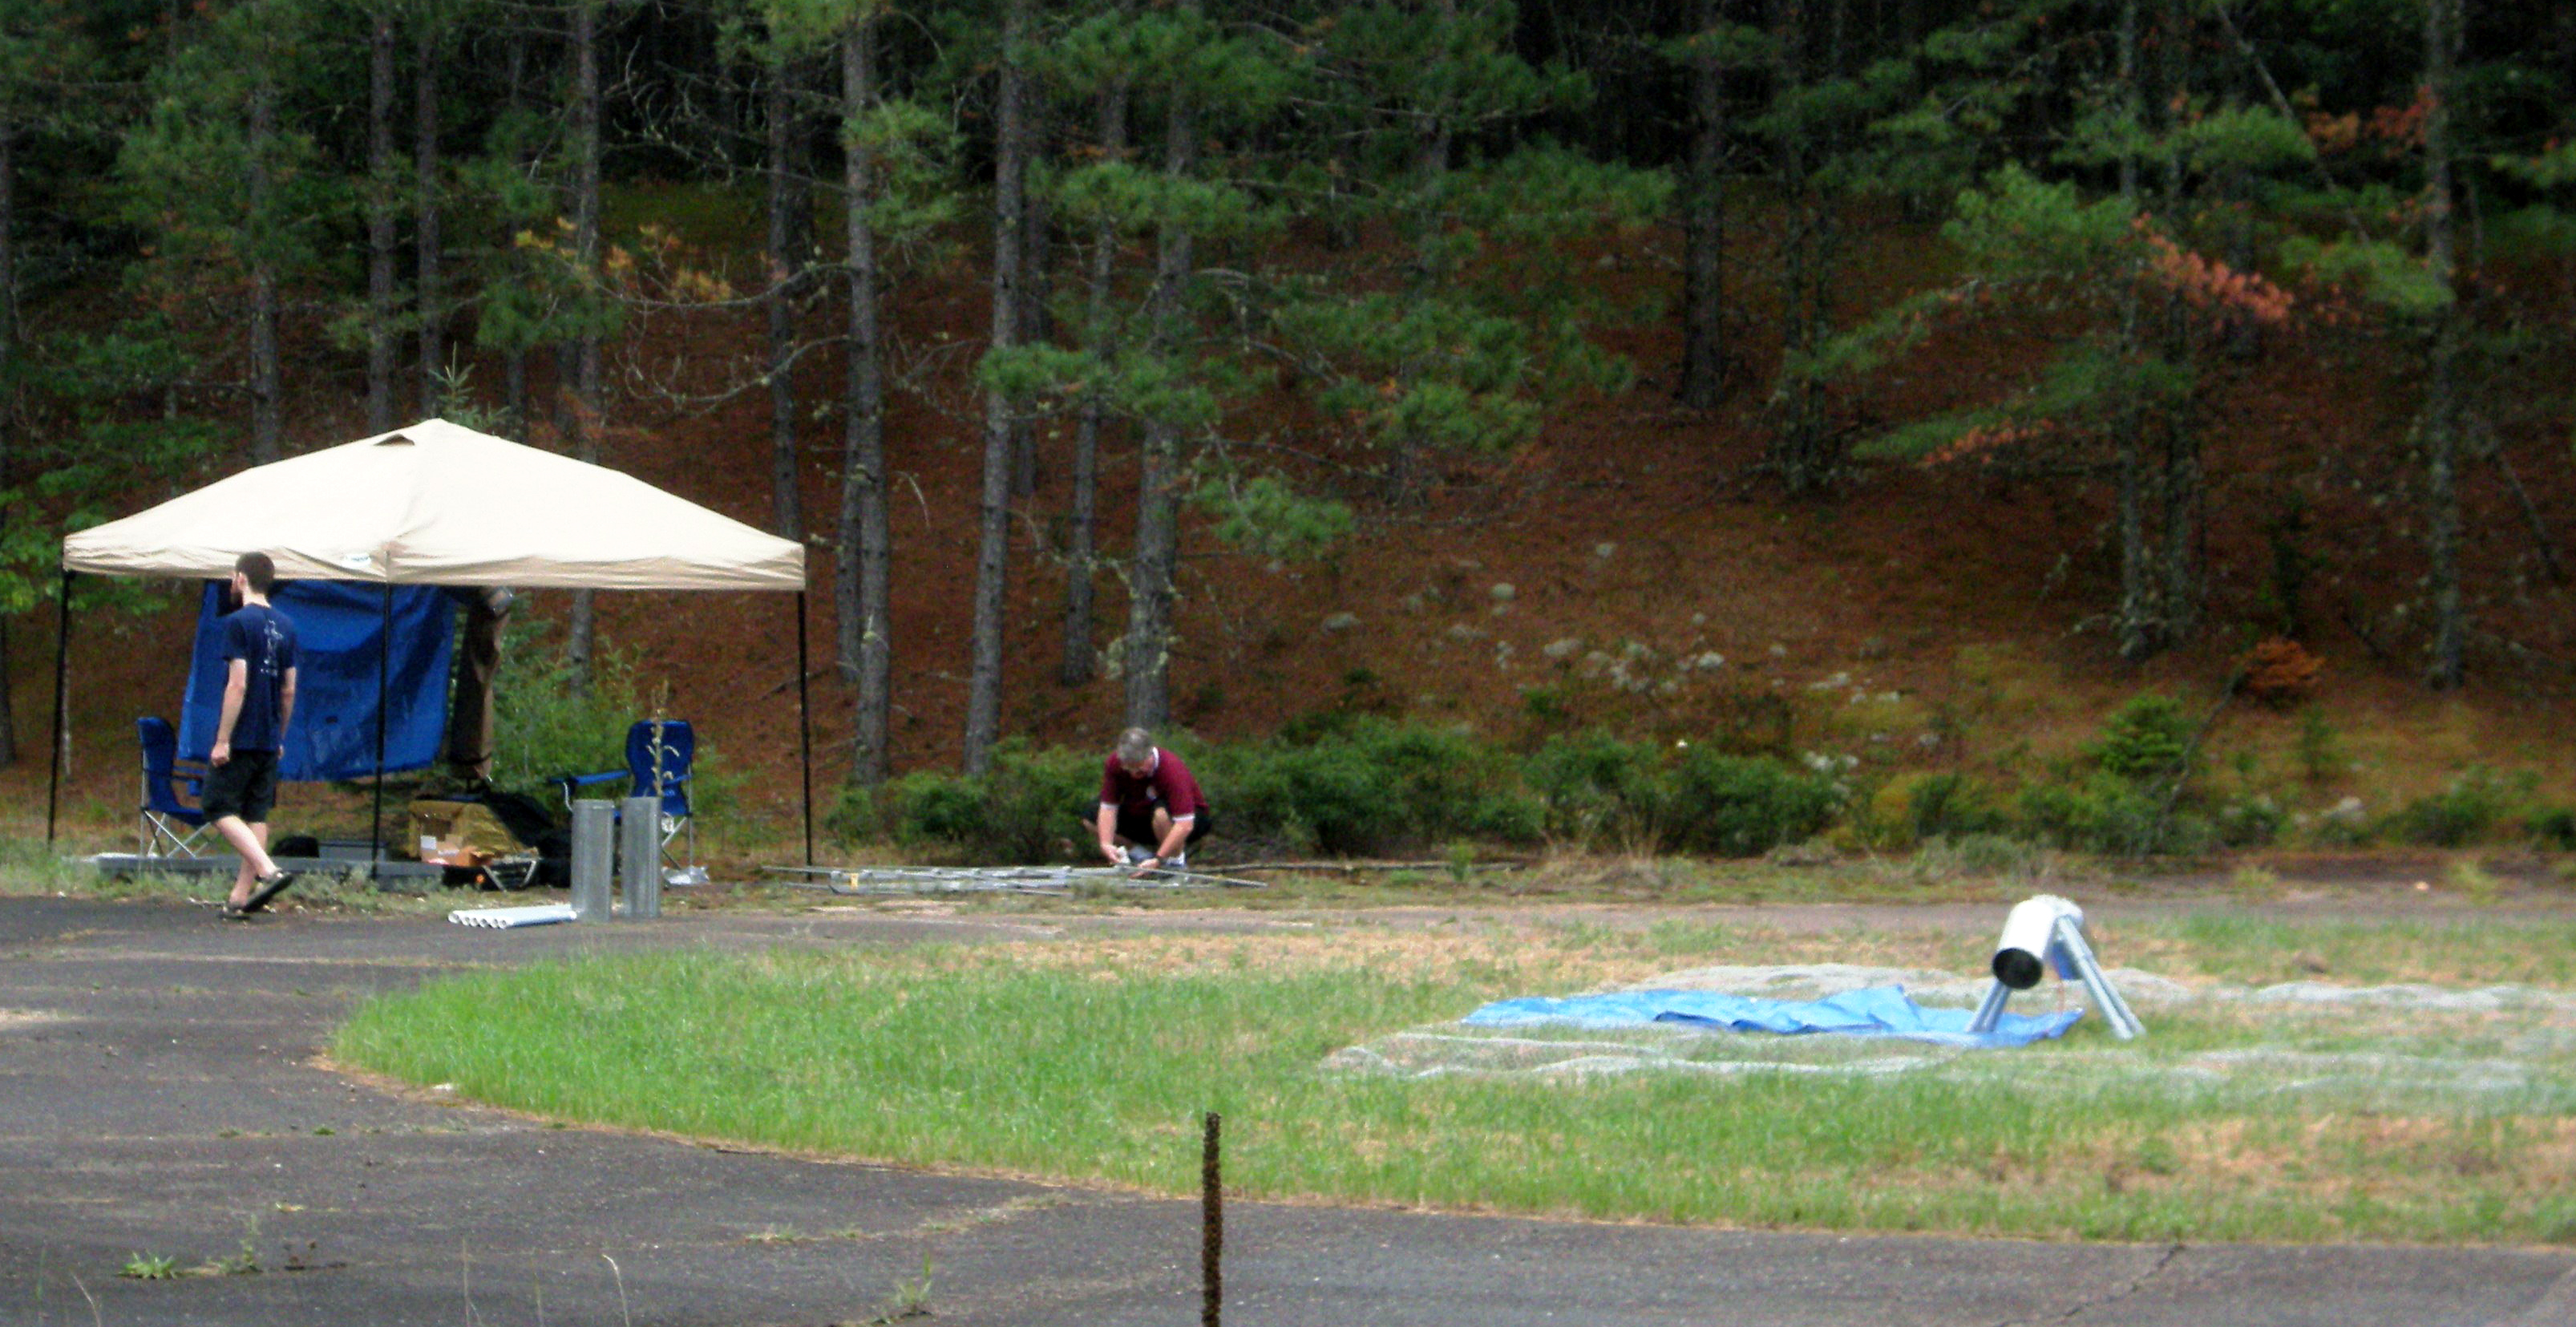
\includegraphics[width=0.95\linewidth]{SCIHI_system/figures/trombone_alg_sys.jpg}
\caption{SCI-HI setup with trombone antenna on site at the Algonquin Radio Observatory in August 2012.}
\label{Fig:trombone_alg}
\end{minipage}%
\begin{minipage}[b]{0.02\textwidth}
\hspace{1cm}
\end{minipage}%
\begin{minipage}[b]{0.42\textwidth}
\centering
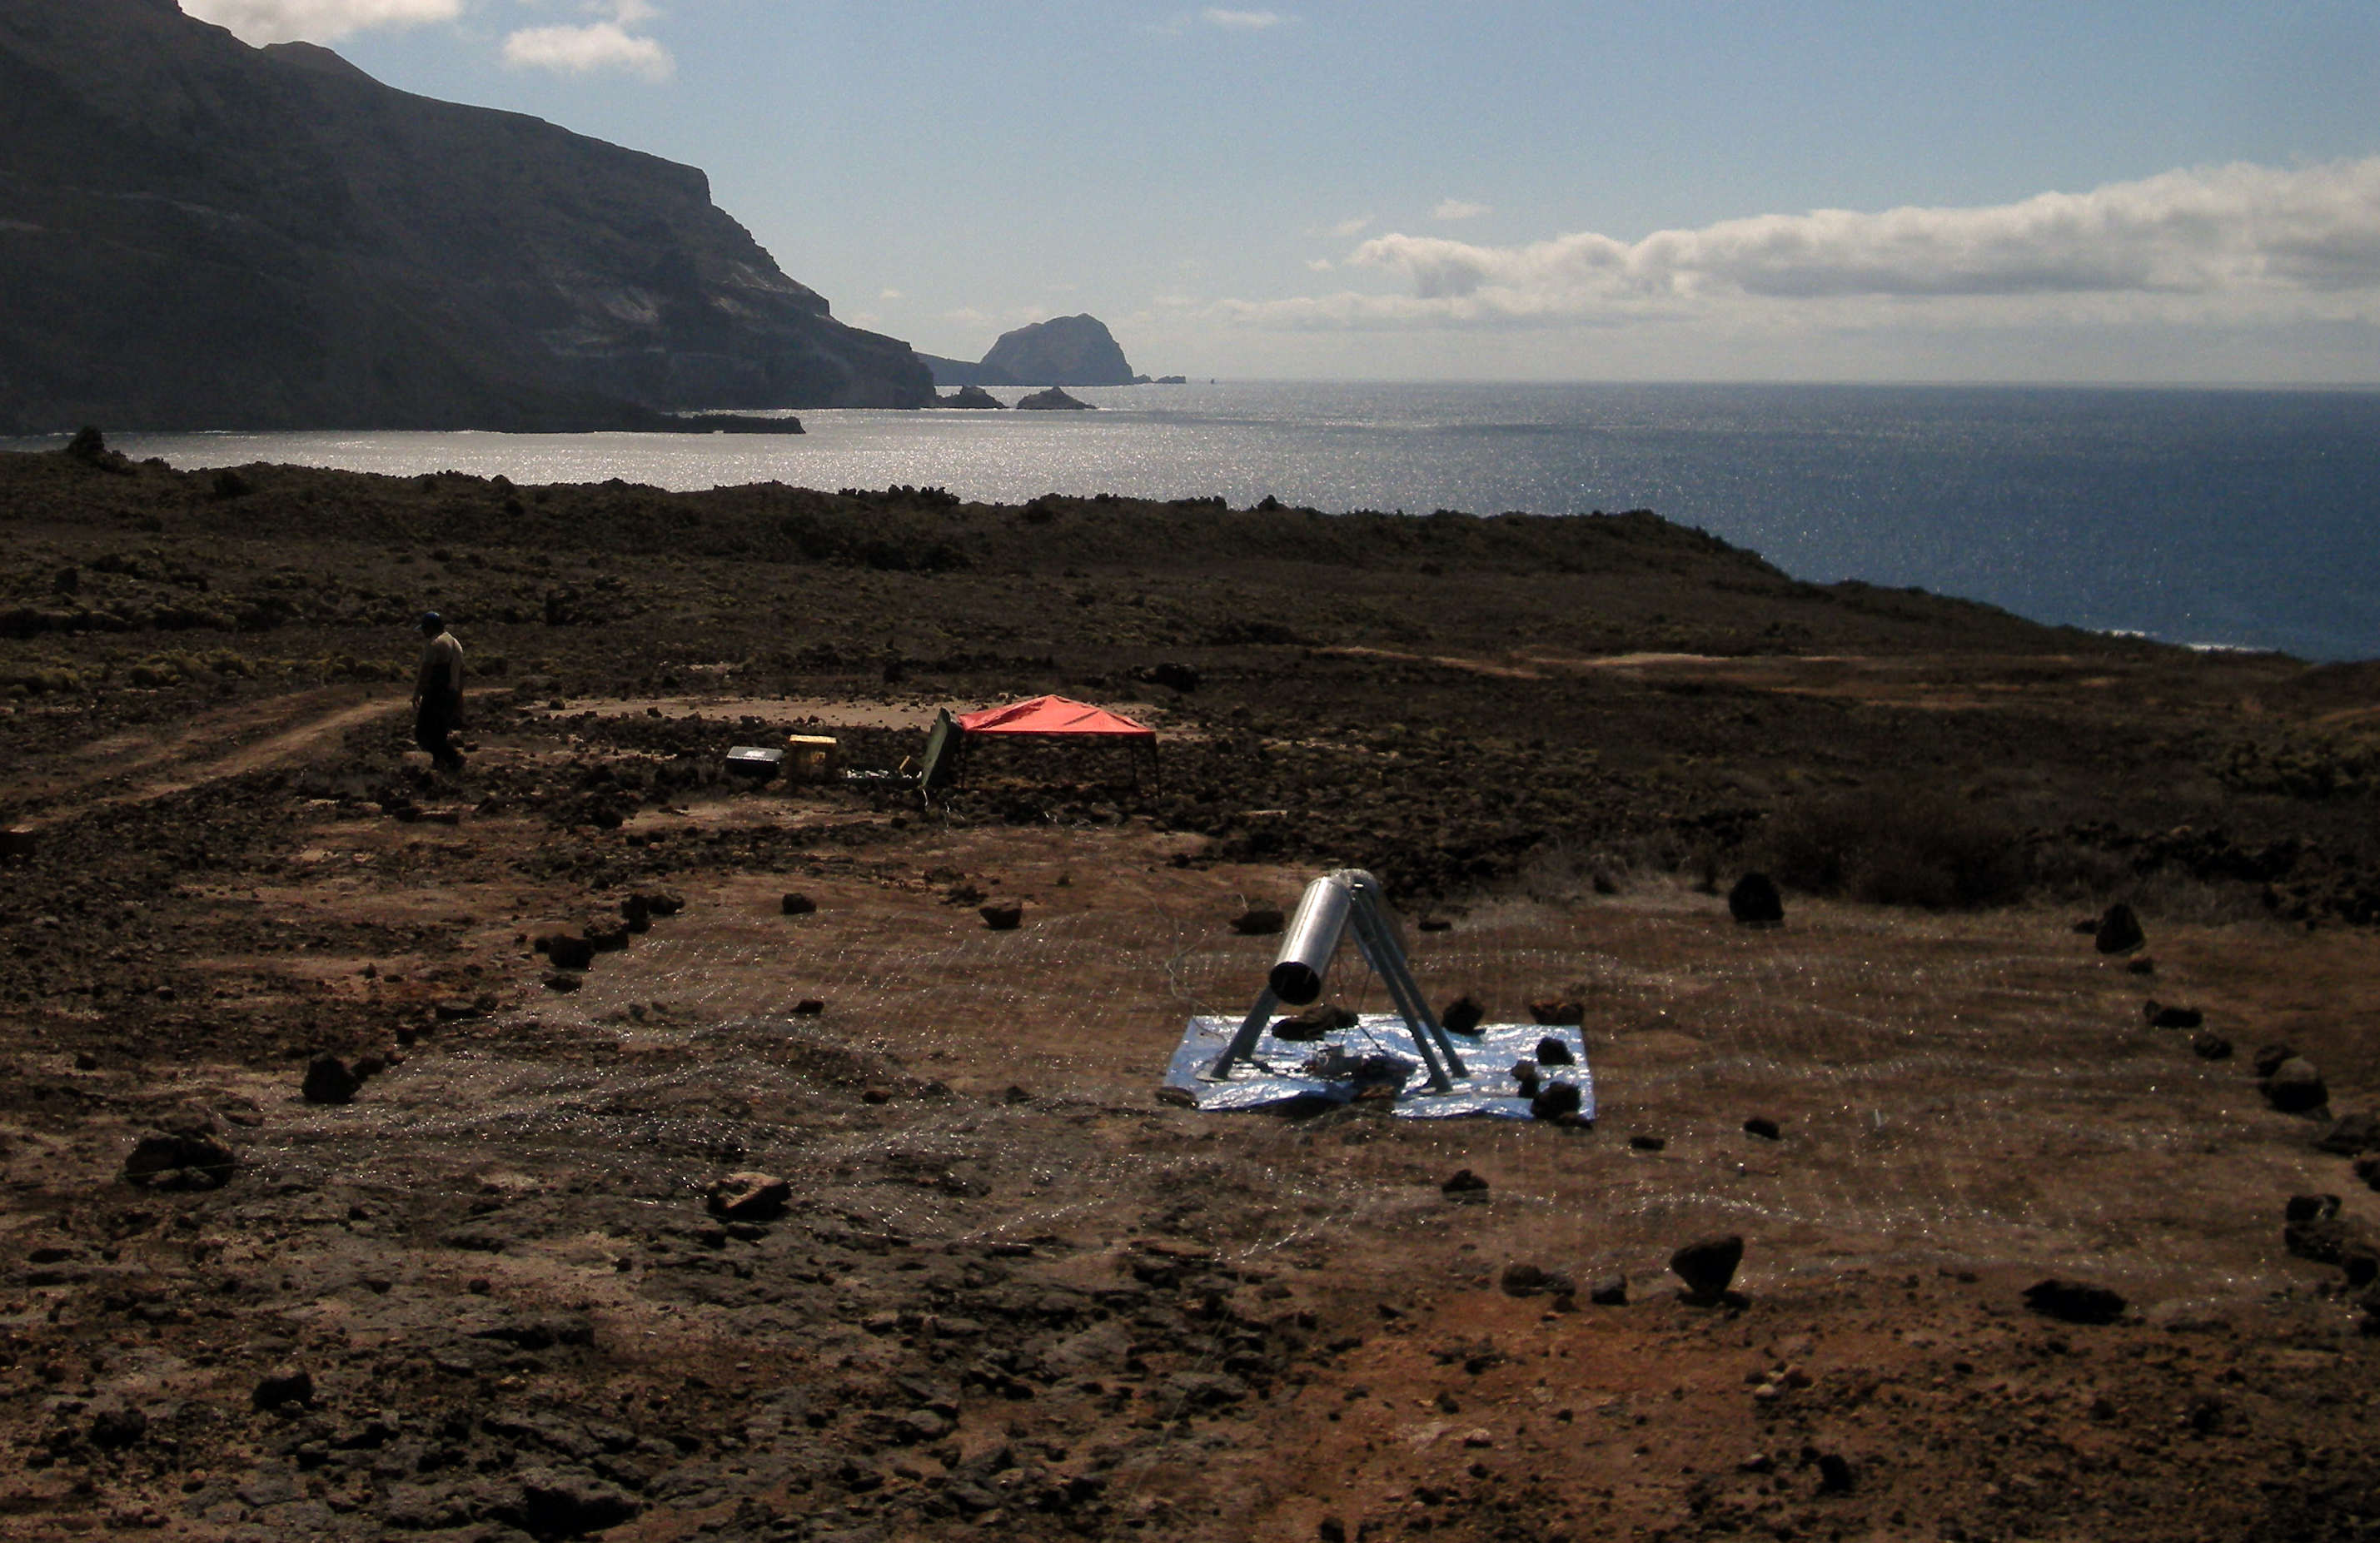
\includegraphics[width=0.95\linewidth]{SCIHI_system/figures/trombone_sys_guad.jpg}
\caption{SCI-HI setup with trombone antenna on site at Isla Guadalupe in October 2012.}
\label{Fig:trombone_guad}
\end{minipage}
\end{figure}

\subsubsection{Antenna Deployment}
The Trombone antenna was used throughout the initial stages of the SCI-HI project, including deployments at Green Bank in West Virginia (Figure \ref{Fig:trombone_gbt}), the Zona del Silencio in Mexico (Figure \ref{Fig:trombone_zds}), Algonquin Radio Observatory in Canada (Figure \ref{Fig:trombone_alg}), and Isla Guadalupe in Mexico (Figure \ref{Fig:trombone_guad}). For more discussion of these sites, see Chapter \ref{Ch:RFI}.

\begin{figure}[htb]
\centering
\begin{minipage}[b]{0.56\textwidth}
\centering
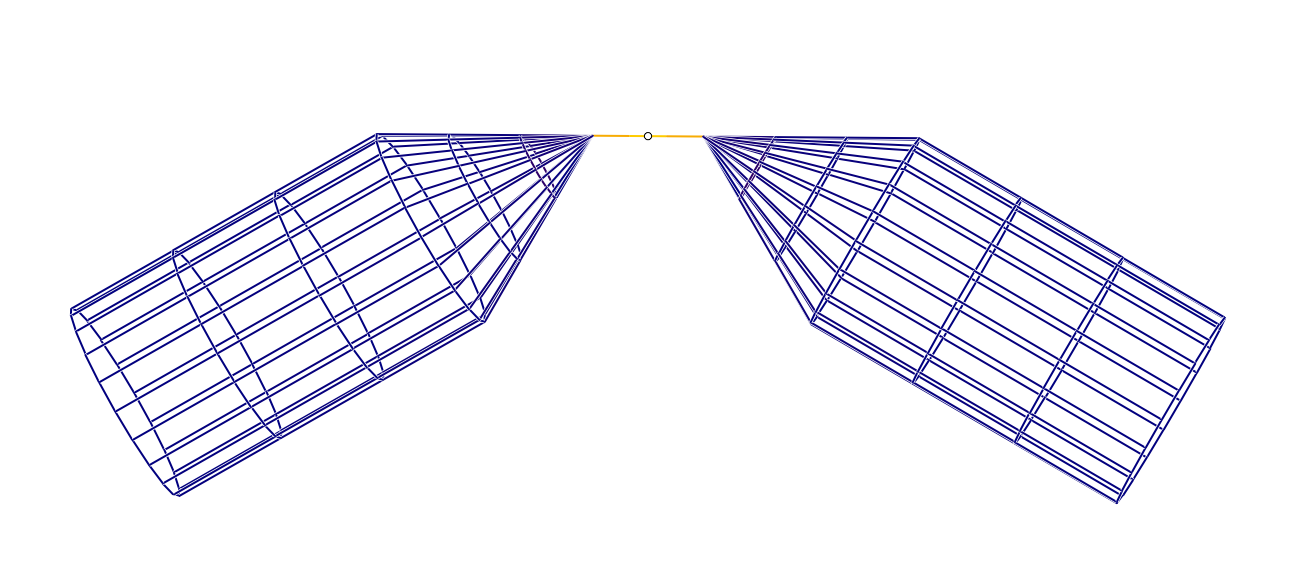
\includegraphics[width=0.95\linewidth]{SCIHI_system/figures/trombone_sim.png}
\caption{Simulated trombone antenna design using cocoaNEC. Simulation software utilizes line segments which intersect to create structures. }
\label{Fig:trombone_sym}
\end{minipage}%
\begin{minipage}[b]{0.02\textwidth}
\hspace{1cm}
\end{minipage}%
\begin{minipage}[b]{0.42\textwidth}
\centering
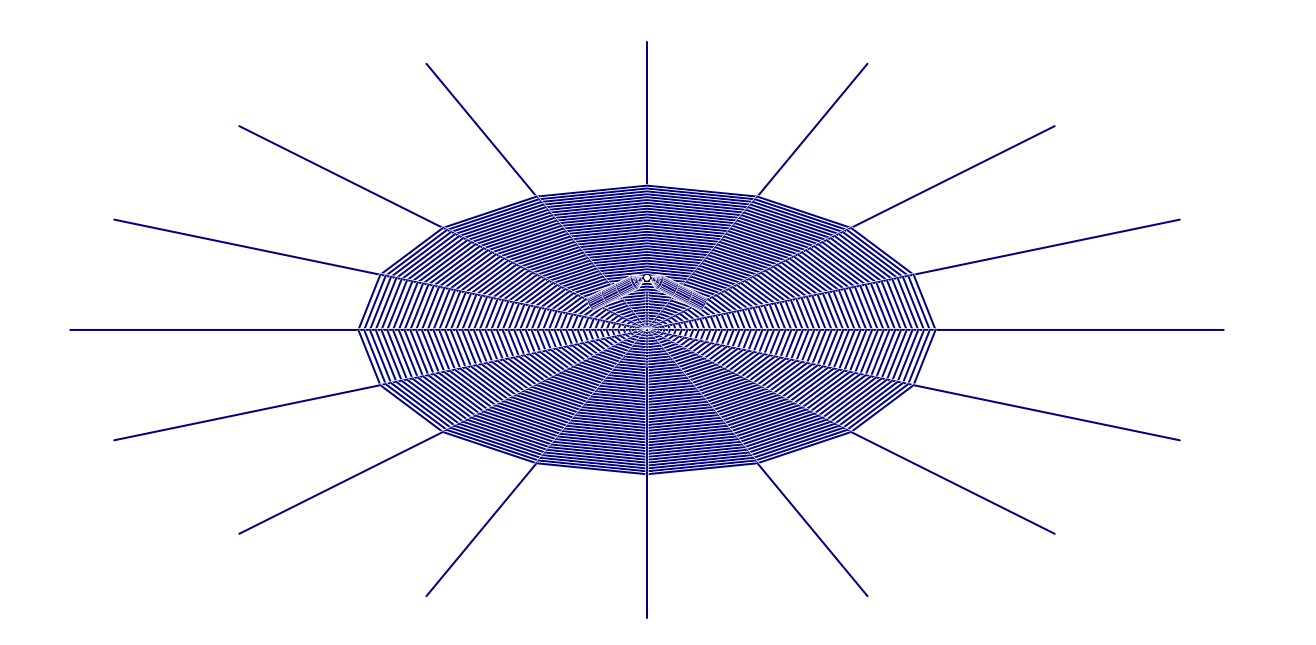
\includegraphics[width=0.95\linewidth]{SCIHI_system/figures/ground_plane_sim.png}
\caption{Circular ground plane with radials, simulated using cocoaNEC. The center, filled section has a 5 meter radius and the radials extend an additional 5 meters.}
\label{Fig:gp_sym}
\end{minipage}
\end{figure}

\begin{figure}[htb]
\begin{center}
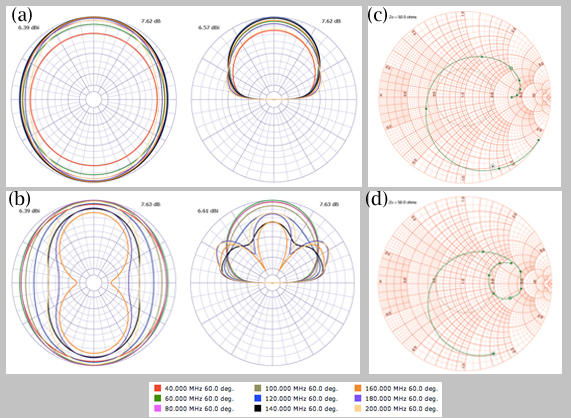
\includegraphics[width=0.95\linewidth]{SCIHI_system/figures/trombone_no_gp.jpg}
\caption{Trombone Simulation results with no ground plane included in the simulation. (a) Shows the azimuth (left) and elevation (right) antenna beam for different frequencies with the antenna at its shortest (35 cm) length. (b) Shows the same plots with the antenna at is longest (86 cm) length. (c) Shows a Smith chart of the antenna complex impedance (S11), where 1.0 is set to $50 \Omega$, for the shortest (35 cm) length. (d) Shows a Smith chart of the antenna complex impedance for the longest (86 cm) length. }
\label{Fig:trsym_nogp}
\end{center}
\end{figure}

\subsubsection{Antenna Simulation}
In order to assess the behavior of the Trombone antenna, simulations were run on the design by Amy Stetten. Figure \ref{Fig:trombone_sym} shows the simulated Trombone design. Simulations were run using cocoaNEC,\footnote{http://www.w7ay.net/site/Applications/cocoaNEC/} a free antenna modelling code designed use in a Macintosh OS environment. 

Simulations showed that the trombone antenna beam was wide, but well behaved for the shorter length as shown in Figure \ref{Fig:trsym_nogp}(a). The longer length antenna beam had quite a bit of structure, as shown in Figure \ref{Fig:trsym_nogp}(b). In addition, the impedance of the antenna (S11) was not well matched to 50 $\Omega$ and varied significantly across the band for all lengths (Figures \ref{Fig:trsym_nogp}(c) and \ref{Fig:trsym_nogp}(d)). 

\begin{figure}[htb]
\begin{center}
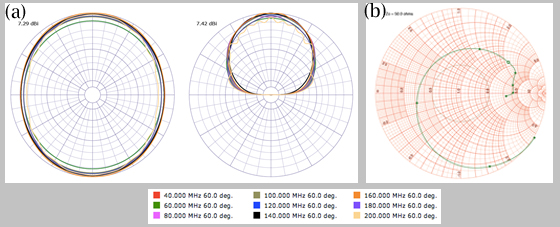
\includegraphics[width=0.95\linewidth]{SCIHI_system/figures/trombone_gp.jpg}
\caption{Trombone Simulation results with spider web ground plane included in the simulation. (a) Shows the azimuth (left) and elevation (right) antenna beam for different frequencies with the antenna at its shortest (35 cm) length. (b) Shows a Smith chart of the antenna complex impedance (S11), where 1.0 is set to $50 \Omega$, for the shortest (35 cm) length.}
\label{Fig:trsym_gp}
\end{center}
\end{figure}

Beyond the trombone design, it was important to examine the effect of a non-infinite ground plane. Preliminary work with a square ground plane led to significant additional structure in the antenna beam. To counteract this structure, the ground plane was modified to the $''$spider-web$''$ design shown in Figure \ref{Fig:gp_sym}, with a center filled region and longer radials. 

Adding this style of ground plane did not have a big impact on the simulation results (see Figure \ref{Fig:trsym_gp}) at most frequencies. There was additional structure in the beam at higher frequencies, but these frequencies are above the target frequency range of 40-130 MHz.  

\begin{figure}[htb]
\centering
\begin{minipage}[b]{0.49\textwidth}
\centering
\includegraphics[width=0.95\linewidth]{SCIHI_system/figures/HIbiscus_top.png}
\caption{Simulated HIbiscus antenna as viewed from above.}
\label{Fig:HI_sim_top}
\end{minipage}%
\begin{minipage}[b]{0.02\textwidth}
\hspace{1cm}
\end{minipage}%
\begin{minipage}[b]{0.49\textwidth}
\centering
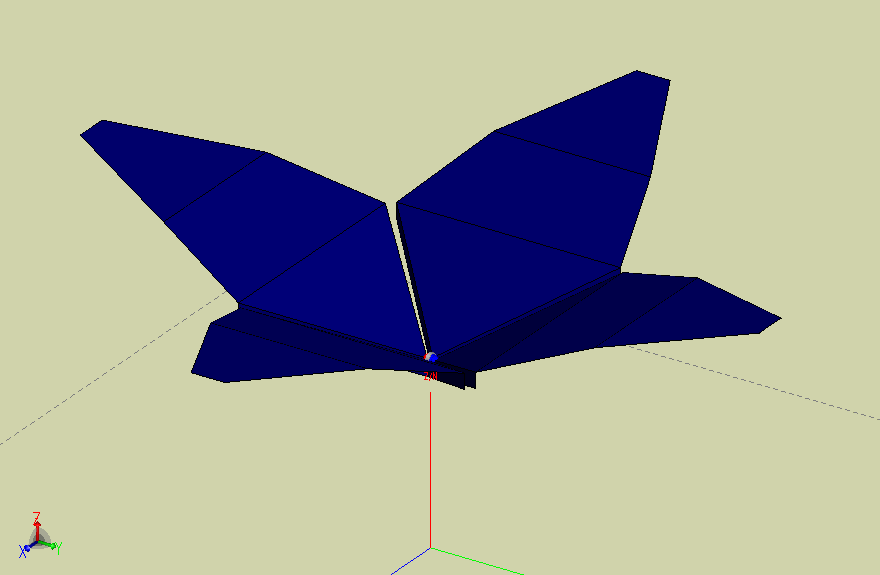
\includegraphics[width=0.95\linewidth]{SCIHI_system/figures/HIbiscus_ISO.png}
\caption{Simulated HIbiscus antenna as viewed from one side.}
\label{Fig:HI_sim_side}
\end{minipage}
\end{figure}

\begin{figure}[htb]
\begin{center}
\includegraphics[width=0.95\linewidth]{SCIHI_system/figures/HIbiscus_gain.png}
\caption{Simulated HIbiscus antenna beam, shown for different frequencies at a single azimuth. The beam is symmetric in azimuth.}
\label{Fig:HIsym_beam}
\end{center}
\end{figure}
 
\begin{figure}[htb]
\centering
\begin{minipage}[b]{0.50\textwidth}
\centering
\includegraphics[width=0.95\linewidth]{SCIHI_system/figures/HIbiscus_S11_50_Cart.png}
\caption{Reflectivity of the simulated HIbiscus antenna when connected to a $50 \Omega$ transmission line. The narrow dip at $\sim 50$ MHz is an antenna resonance. }
\label{Fig:HIsim_S11_dB}
\end{minipage}%
\begin{minipage}[b]{0.02\textwidth}
\hspace{1cm}
\end{minipage}%
\begin{minipage}[b]{0.46\textwidth}
\centering
\includegraphics[width=0.95\linewidth]{SCIHI_system/figures/HIbiscus_S11_50_Smith.png}
\caption{Smith chart of the simulated HIbiscus antenna complex S11 relative to $50 \Omega$ for 30 - 180 MHz.}
\label{Fig:HIsim_S11_Smith}
\end{minipage}
\end{figure}

\subsection{HIbiscus Antenna Design}

Simulation and testing demonstrated that the trombone design had a wide beam that was not well behaved at higher frequencies. In addition, the impedance of the antenna was complex and strongly varying over our frequency band. 

Because of these problems, we decided to shift our antenna design in a new direction based upon our expectations from the literature (\textcolor{red}{Need to add specific references for different antenna types}). We tested several antenna designs in simulation, including the four-square design used in the EDGES experiment \cite{rogers_2012}. Simulations were run by Jose-Miguel Juaregui-Garcia using FEKO, a finite element computational electromagnetics software package.\footnote{https://www.feko.info/} 

Based on the FEKO simulation results we settled on a design that used the EDGES design as a starting point, but changed the exact shapes of the four squares. We took each square and turned it into an incliclined petal composed of three trapezoidal shapes. Each shape was connected to its neighbors on the petal, but had a different angle with respect to the ground. Additional panels were added to each side of the petal to create a strip line with a fixed gap between the petals. The entire antenna was then placed above a flat ground plane. We call this design a HIbiscus antenna, as shown in Figures \ref{Fig:HI_sim_top} and \ref{Fig:HI_sim_side}. 

This HIbiscus design has an azimuthally symmetric beam with a $\sim 55^\circ$ full width half-maximum (FWHM) and no sidelobes over a wide frequency band, as shown in Figure \ref{Fig:HIsym_beam}. The impedance of the HIbiscus antenna is complex, but is centered around 50 $\Omega$ such that it has less than $-10 dB$ of reflectivity over 60 MHz. The simulated complex simulated impedance is shown in Figure \ref{Fig:HIsim_S11_Smith}, and the simulated antenna reflectivity is shown in Figure \ref{Fig:HIsim_S11_dB}. 

\begin{figure}[htb]
\centering
\begin{minipage}[b]{0.50\textwidth}
\centering
\includegraphics[width=0.95\linewidth]{SCIHI_system/figures/model_test_tabitha.jpg}
\caption{Testing a model HIbiscus antenna in the CMU Project REAL Chamber. }
\label{Fig:hibiscus_scale_tabitha}
\end{minipage}%
\begin{minipage}[b]{0.02\textwidth}
\hspace{1cm}
\end{minipage}%
\begin{minipage}[b]{0.44\textwidth}
\centering
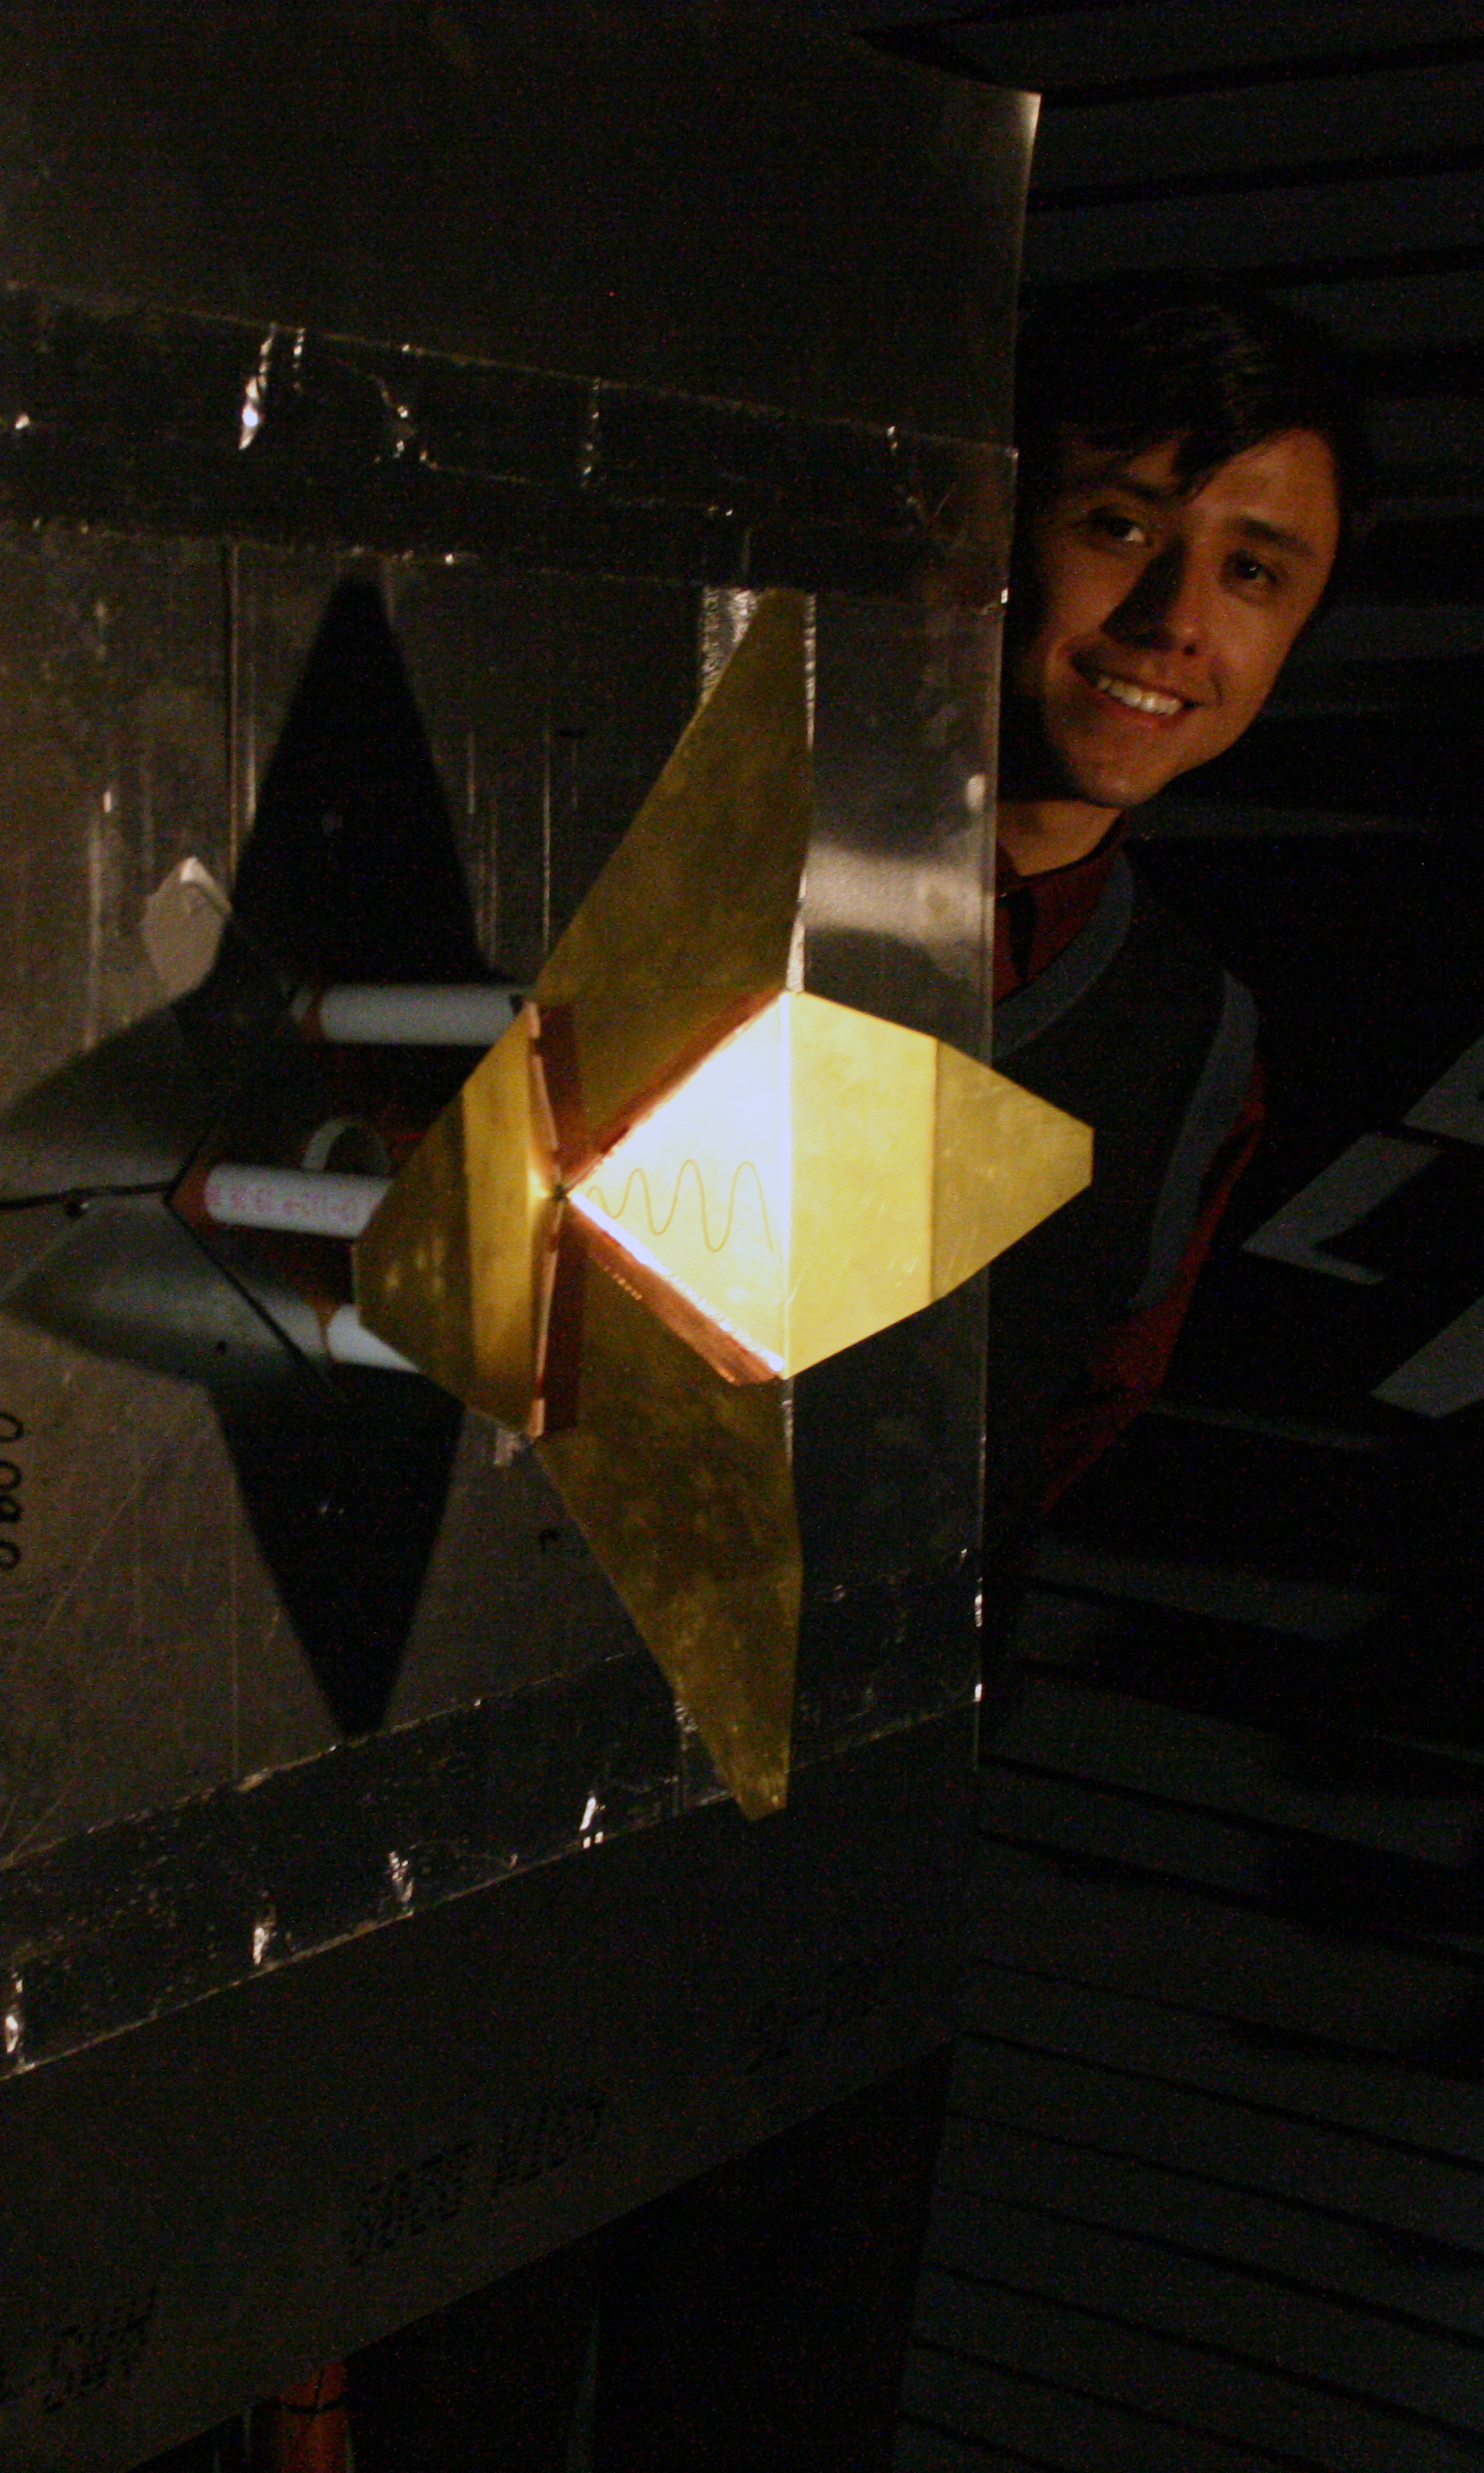
\includegraphics[width=0.95\linewidth]{SCIHI_system/figures/model_test_jose.jpg}
\caption{Scale model test with a different HIbiscus antenna model.}
\label{Fig:hibiscus_scale_jose}
\end{minipage}
\end{figure}

\subsubsection{Scale Model Testing}
In order to test our simulation to see if it matched the real antenna performance, Jose-Miguel built a set of scaled HIbiscus designs tuned for higher frequencies around 400-500 MHz. This allowed us to use an antenna range to measure the antenna beam shape and S-parameters. 

Jose-Miguel and I used the Project REAL\footnote{http://www.preal.ece.cmu.edu/} (Remote Educational Antenna Laboratory) facility at Carnegie Mellon University to measure the antenna response of different scaled HIbiscus models, as is shown in Figures \ref{Fig:hibiscus_scale_tabitha} and \ref{Fig:hibiscus_scale_jose}. 

This scale model testing indicated that the shape parameters that were most significant in affecting antenna performance were the strip line gap width and the height of the antenna with respect to the ground plane. By incrementally adjusting these parameters on the scale models, we were able to tune the antenna scale model to optimize these critical parameters in a real design. 

Using the scale model data, Jose-Miguel was also able to edit the antenna simulation to better match the actual antenna response, providing us with an antenna simulation dataset that was closer to reality. 

\begin{figure}[htb]
\centering
\begin{minipage}[b]{0.43\textwidth}
\centering
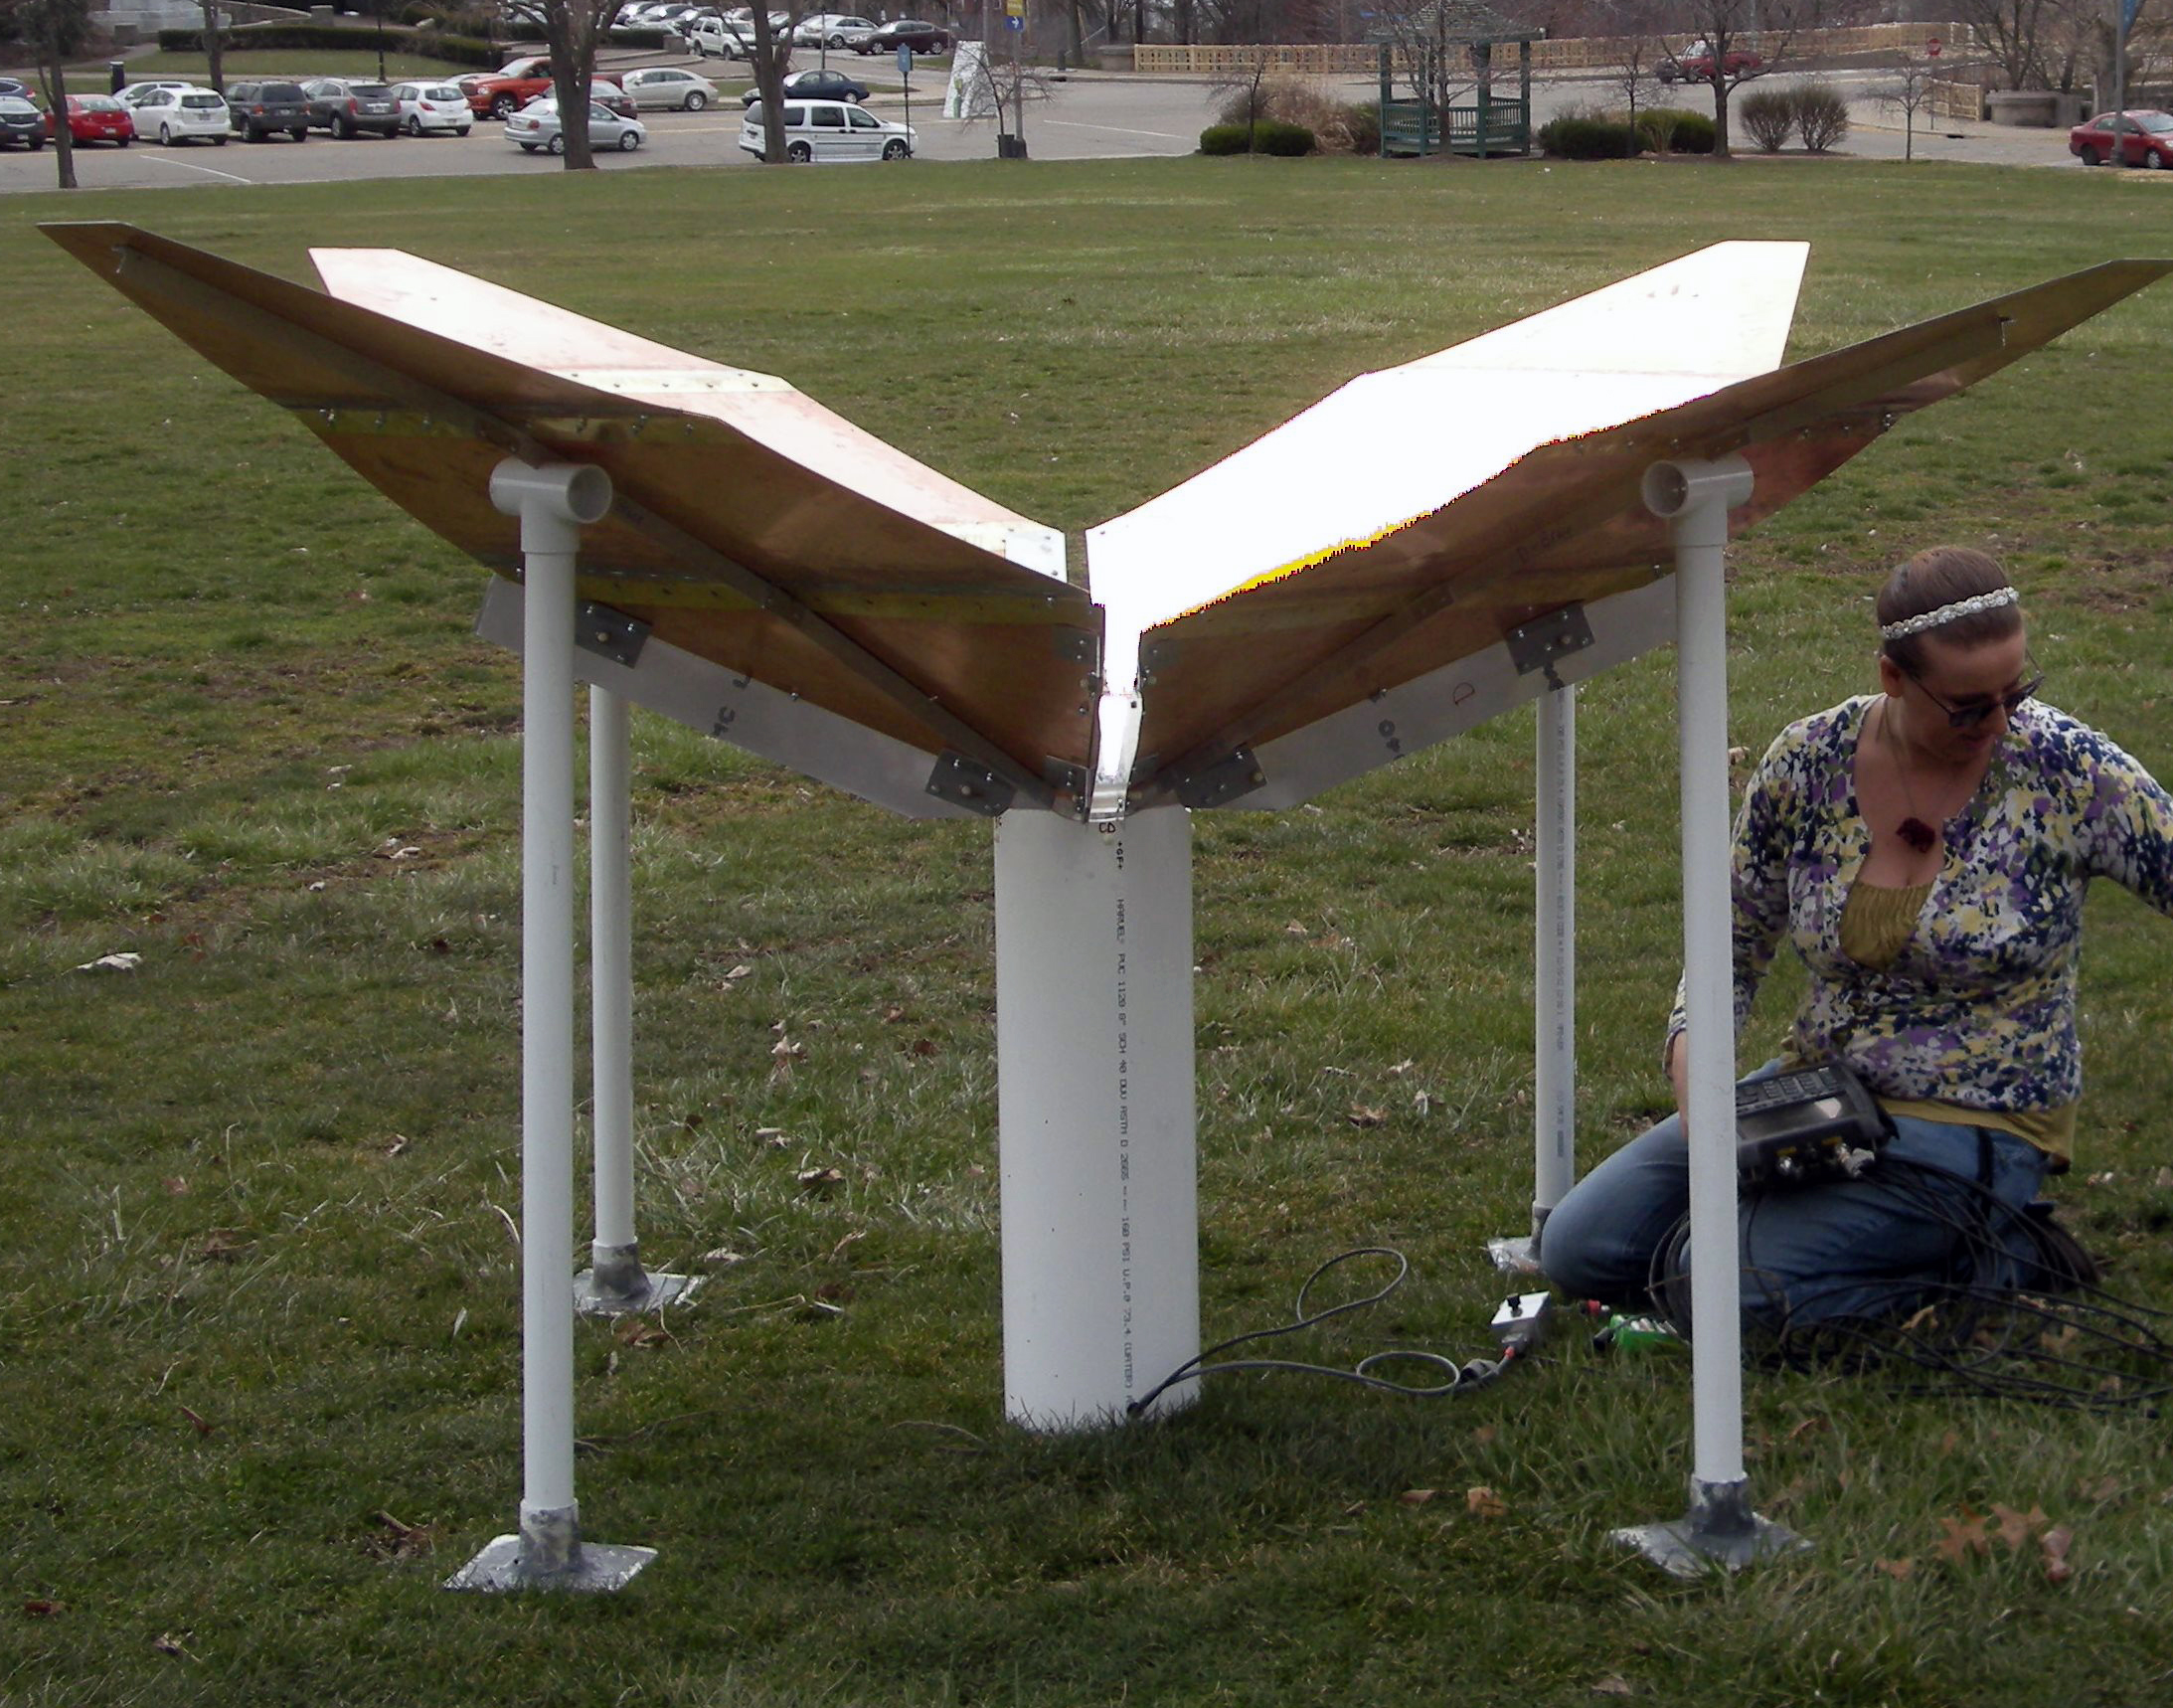
\includegraphics[width=0.95\linewidth]{SCIHI_system/figures/HIbiscus_pgh_imp.jpg}
\caption{HIbiscus antenna scaled for 70 MHz as it was setup during S-parameter testing at CMU. }
\label{Fig:hibiscus_first}
\end{minipage}%
\begin{minipage}[b]{0.02\textwidth}
\hspace{1cm}
\end{minipage}%
\begin{minipage}[b]{0.51\textwidth}
\centering
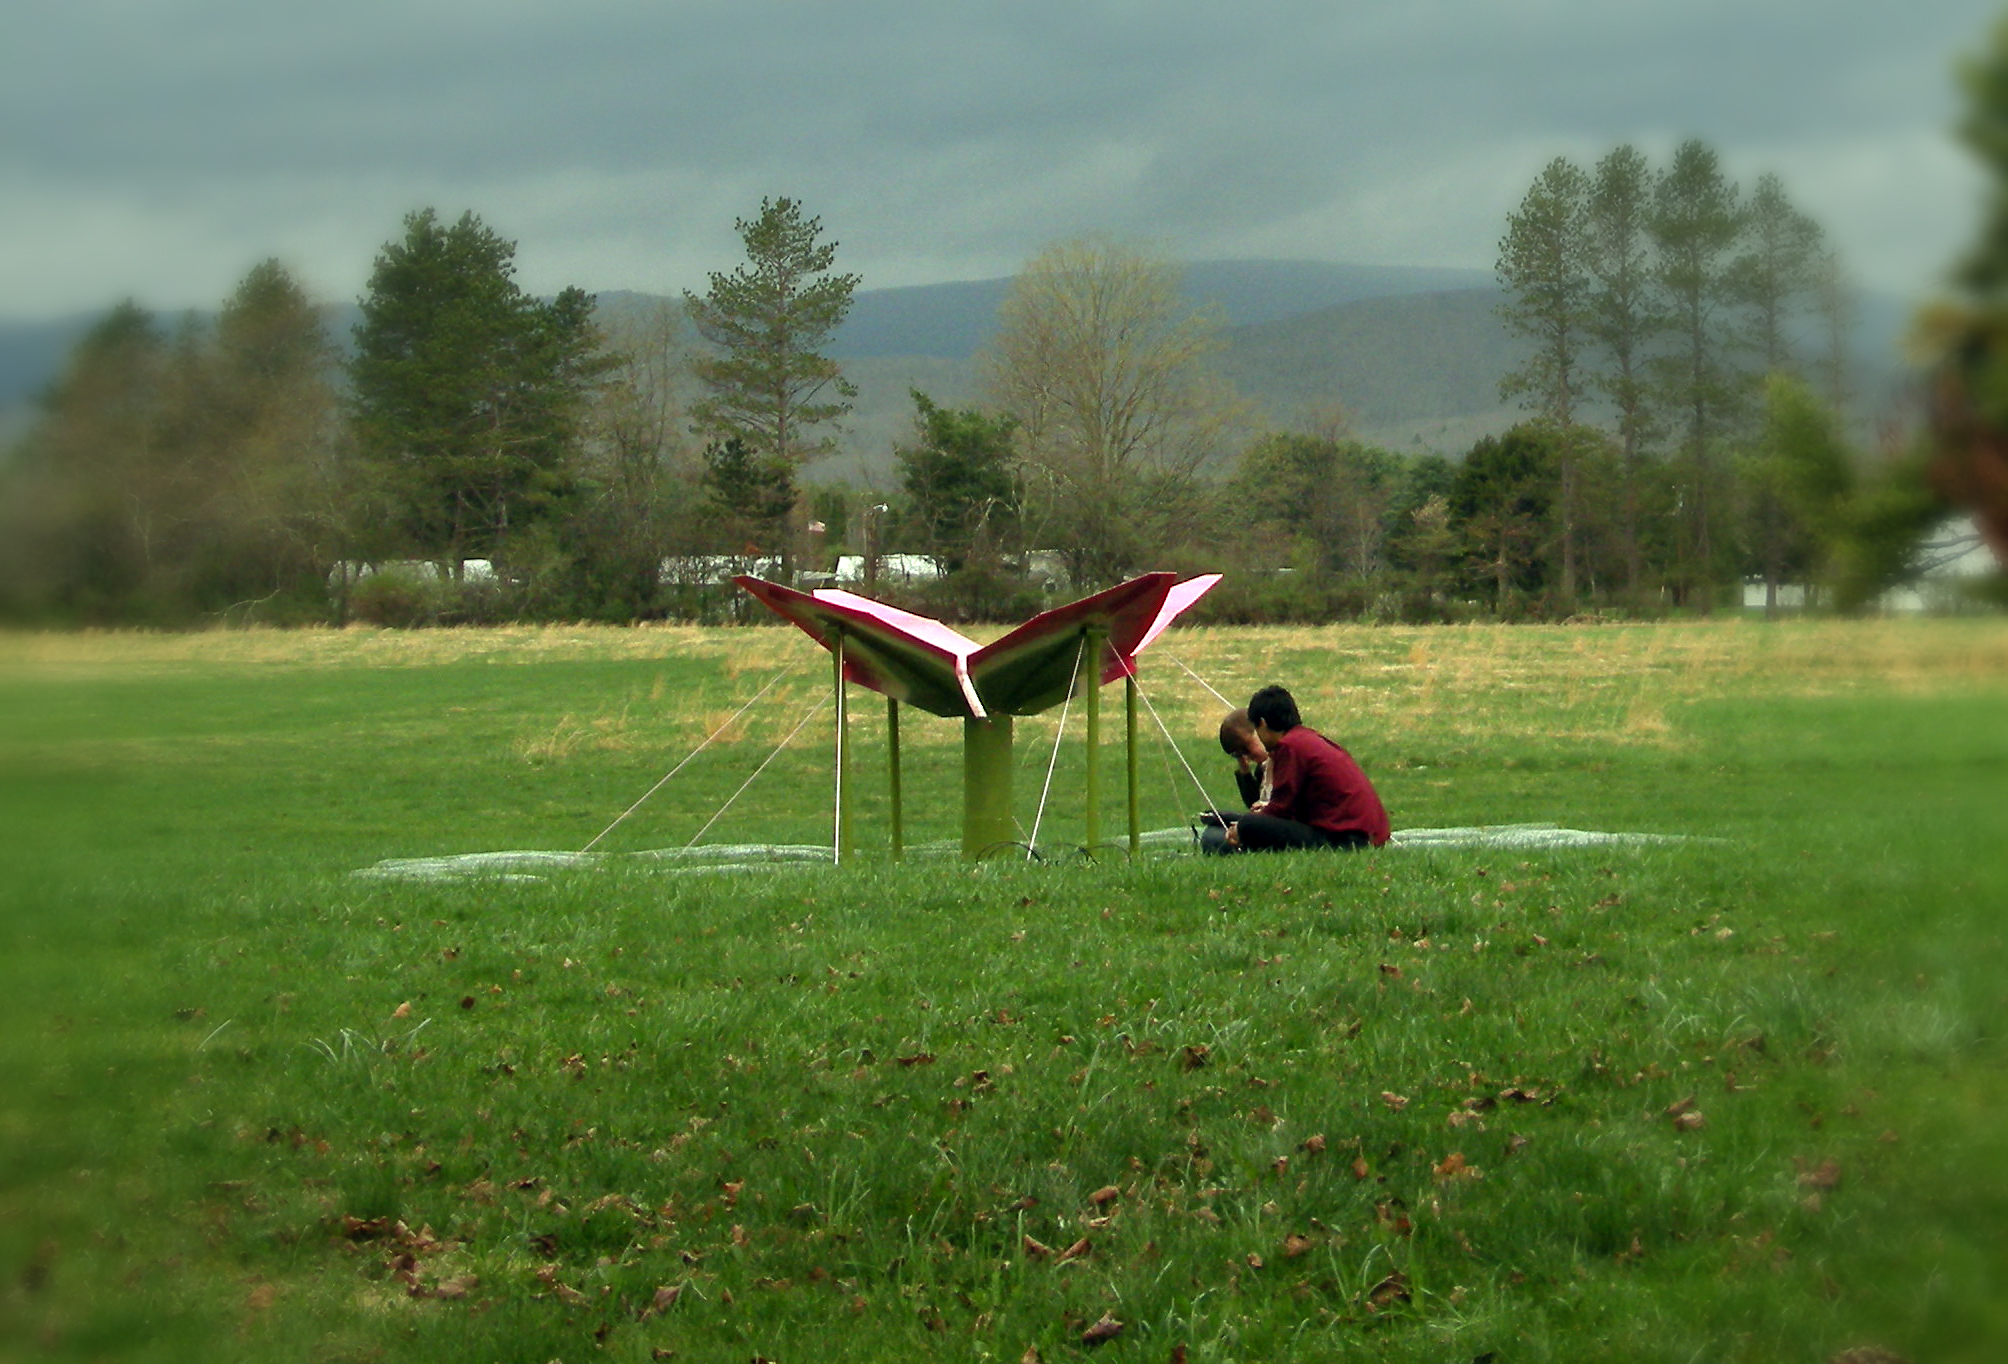
\includegraphics[width=0.95\linewidth]{SCIHI_system/figures/HIbiscus_gbt.jpg}
\caption{HIbiscus antenna scaled for 70 MHz setup for s-parameter testing on site at Green Bank.}
\label{Fig:hibiscus_gbt}
\end{minipage}
\end{figure}

\subsection{HIbiscus Antenna Construction}

\subsubsection{Initial Assembly}
Once we had a design finalized, Jose-Miguel and I set out to construct a HIbiscus antenna with its center frequency tuned to 70 MHz (in the middle of the SCI-HI observation band).

To construct the antenna petals, we started with large sheets of printed circuit board (pcb) material (see Figure \ref{Fig:hibiscus_pcb}). This material is a sheet of fiberglass sandwiched by two thin sheets of copper. We cut each of the trapezoidal shapes out of the pcb material, then added brass flanges to connect the shapes. Underneath the center line of each petal we placed a rib made out of aluminum angle with the appropriate bends to match the angles between trapezoids. Finally, the strip line panels were added using brass sheets soldered to some of the trapezoids (see Figure \ref{Fig:hibiscus_solder}). The entire system is bolted together using screws, and can be separated into parts for travel. 

\begin{figure}[htb]
\centering
\begin{minipage}[b]{0.39\textwidth}
\centering
\includegraphics[width=0.95\linewidth]{SCIHI_system/figures/HIbiscus_pcb_cut.jpg}
\caption{HIbiscus antenna pcb panels being cut. }
\label{Fig:hibiscus_pcb}
\end{minipage}%
\begin{minipage}[b]{0.02\textwidth}
\hspace{1cm}
\end{minipage}%
\begin{minipage}[b]{0.55\textwidth}
\centering
\includegraphics[width=0.95\linewidth]{SCIHI_system/figures/HIbiscus_solder.jpg}
\caption{Soldering the strip line to the HIbiscus antenna panels.}
\label{Fig:hibiscus_solder}
\end{minipage}
\end{figure} 

In order to keep the petal separation even and correct, lucite spacers were placed between each of the petals (see Figure \ref{Fig:hibiscus_spacer}). In addition, a lucite mount was built for the connection points at the center of the antenna (see Figure \ref{Fig:hibiscus_center}). The entire system was raised above the ground using a set of five PVC pipe legs; a central column and one leg for each petal (see Figure \ref{Fig:hibiscus_first}). 

\begin{figure}[htb]
\centering
\begin{minipage}[b]{0.52\textwidth}
\centering
\includegraphics[width=0.95\linewidth]{SCIHI_system/figures/HIbiscus_strip_line.jpg}
\caption{Sight line down one of the strip lines for the HIbiscus antenna with spacers in place.}
\label{Fig:hibiscus_spacer}
\end{minipage}%
\begin{minipage}[b]{0.02\textwidth}
\hspace{1cm}
\end{minipage}%
\begin{minipage}[b]{0.42\textwidth}
\centering
\includegraphics[width=0.95\linewidth]{SCIHI_system/figures/HIbiscus_center_point.jpg}
\caption{Center of the HIbiscus antenna with spacers and center mount block in place.}
\label{Fig:hibiscus_center}
\end{minipage}
\end{figure}

Beyond the antenna structure, a ground plane was also required to avoid variation in the antenna pattern and impedance due to weather conditions. Like with the Trombone, we used a ground plane made out of chicken wire. In this case, our simulations showed us that a $\sim 100 m^2$ square ground plane was sufficient for our application. The entire system (antenna plus ground plane) was anchored to the ground to minimize the wind impact on the system. Each of the four support legs had an anchoring rope (see Figure \ref{Fig:hibiscus_gbt}), and the chicken wire was also anchored with many stakes. 

\subsubsection{S-parameters and Impedance}\label{Sec:HIbiscus_Imp}

With the antenna constructed, we could test that it matched our scale model measurements in terms of its S-parameters. To do this, we set up the antenna outdoors and made measurements with a portable Vector Network Analyzer (VNA). Measurements had to be made outdoors because the wavelengths corresponding to the SCI-HI frequencies ($40-130$ MHz) are $\sim$1-10 meters. This large wavelength scale means that reflections from the boundaries of a room can change antenna s-parameters, so accuracy in measurement requires the outdoor setting. Figures \ref{Fig:hibiscus_first} and \ref{Fig:hibiscus_gbt} show examples of how we made this measurement at CMU and Green Bank.

\textcolor{red}{Here I'll add a discussion of HIbiscus S11 data using VNA and explanation, along with figures showing the structures.}

\subsubsection{Travelling with the Antenna}
In order to use the HIbiscus antenna on-site at remote locations, it needed to be transportable to those locations and easily assembled upon arrival. The physical construction of the antenna was designed to match this requirement in a number of ways. 

First, the entire system was made as lightweight as possible. This was accomplished by using the pcb material, which was much lighter and stiffer than the equivalent sheet metal panels would be. 

Second, the system was designed in segments so it could be assembled and disassembled and packed into small bags. Each petal separated out into three trapezoids that were screwed together for assembly, but could be packed as mostly flat sheets. The lucite spacers and mount were attached to the petals using screws and could be removed and packed for travel, as were the PVC pipe supports. 

Third, the entire system was arranged for travel in three suitcases (plus an extra bag for the ground plane chicken wire). These suitcases were small and light enough to be checked as regular baggage on commercial airlines. 

\begin{figure}[htb]
\begin{center}
%\centering
%\begin{minipage}[b]{0.47\textwidth}
%\centering
\includegraphics[width=0.95\linewidth]{SCIHI_system/figures/HIbiscus_70mhz_lab.jpg}
\caption{New HIbiscus antenna scaled for 70 MHz as laid out in the lab. Scale model in picture for comparison.}
\label{Fig:hibiscus_70}
\end{center}
\end{figure}

%\end{minipage}%
%\begin{minipage}[b]{0.02\textwidth}
%\hspace{1cm}
%\end{minipage}%
%\begin{minipage}[b]{0.47\textwidth}
%\centering

\begin{figure}[htb]
\begin{center}
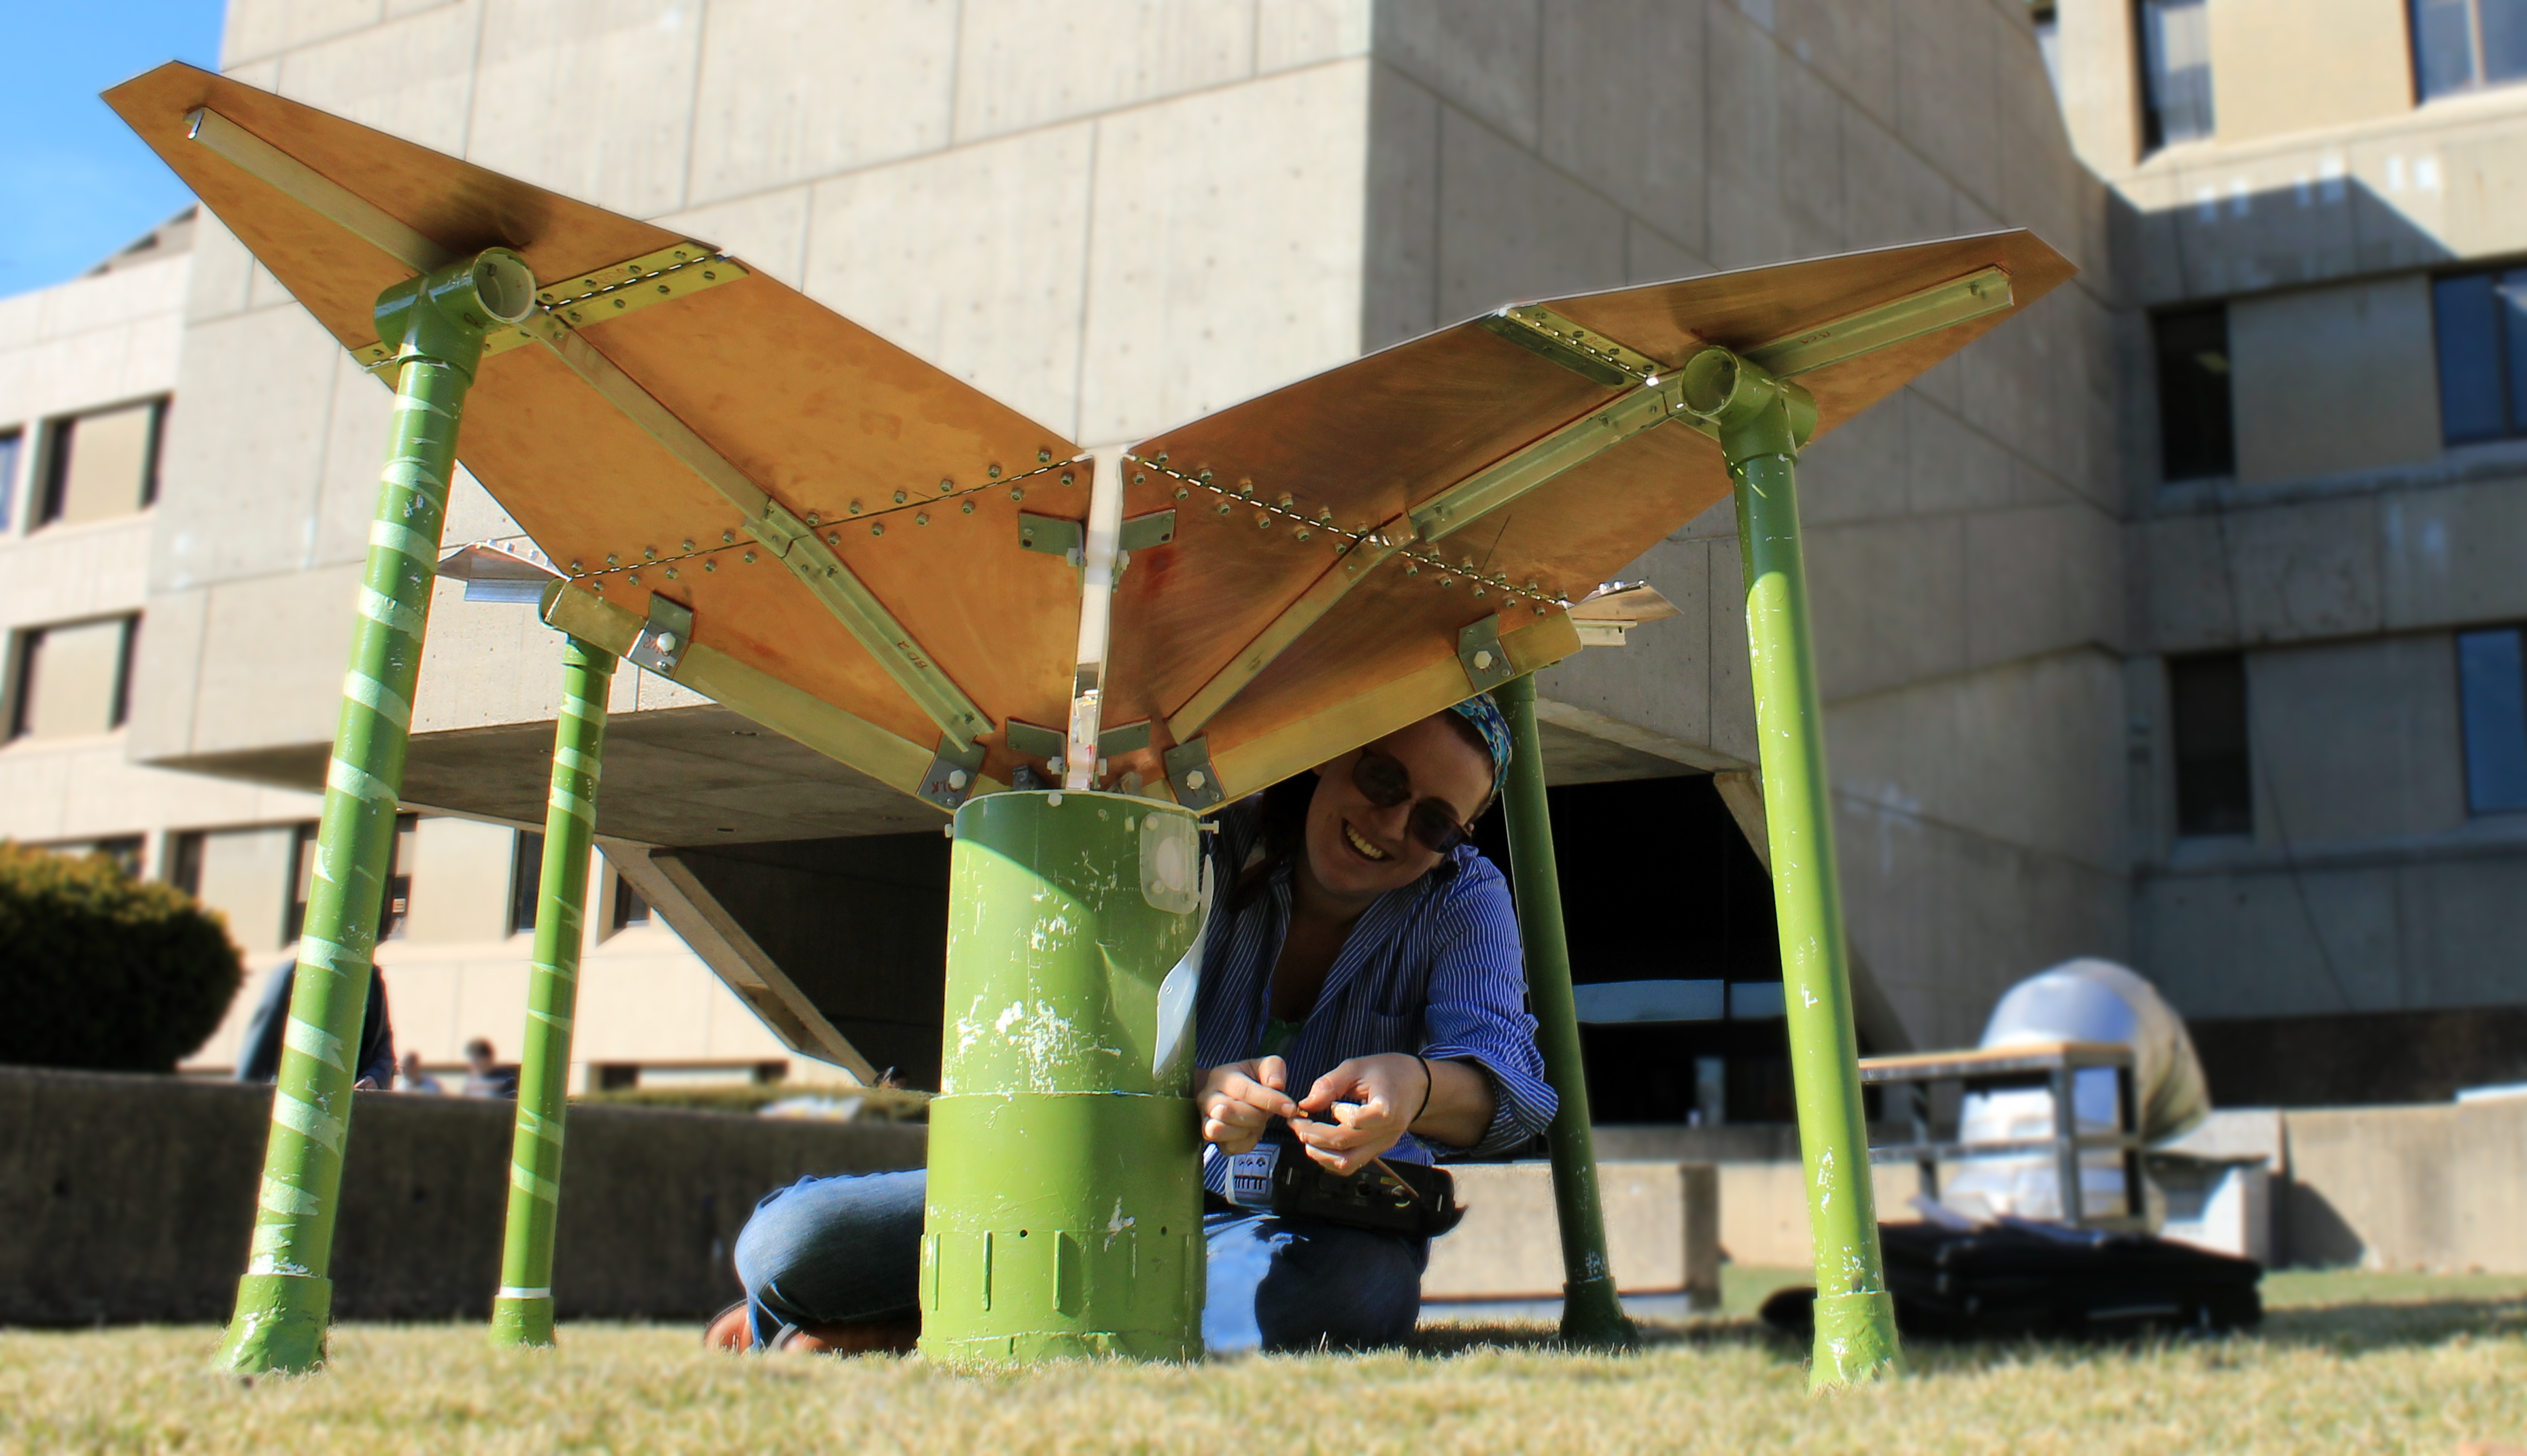
\includegraphics[width=0.95\linewidth]{SCIHI_system/figures/HIbiscus_100mhz.jpg}
\caption{New HIbiscus antenna scaled for 100 MHz as set up on the lawn at CMU while its S-parameters were measured. }
\label{Fig:hibiscus_100}
%\end{minipage}
\end{center}
\end{figure}

\subsubsection{Antenna Upgrades}
Deployment of the SCI-HI system in June 2013 demonstrated that the HIbiscus antenna could use some improvements prior to future deployements. The first and most significant change was the addition of a second antenna scaled to have a center frequency of 100 MHz. By having both scales (70 MHz and 100 MHz), data can now be collected over a wider range of frequencies. In addition, the overlap region where both antennas work ($\sim 85-95$ MHz) provides a cross check for the signal. In other words, this cross check will help us to make sure that any spectral structure measured is not coming from the antenna. 

\begin{figure}[htb]
\centering
\begin{minipage}[b]{0.33\textwidth}
\centering
\includegraphics[width=0.95\linewidth]{SCIHI_system/figures/HIbiscus_petals.jpg}
\caption{HIbiscus petals with hinged joints.}
\label{Fig:hibiscus_petal}
\end{minipage}%
\begin{minipage}[b]{0.02\textwidth}
\hspace{1cm}
\end{minipage}%
\begin{minipage}[b]{0.61\textwidth}
\centering
\includegraphics[width=0.95\linewidth]{SCIHI_system/figures/HIbiscus_folded_70mhz.jpg}
\caption{HIbiscus petals folded up in preparation for packing.}
\label{Fig:hibiscus_fold}
\end{minipage}
\end{figure}

We built a new 70 MHz antenna (see Figure \ref{Fig:hibiscus_70}) as well as the 100 MHz antenna (see Figure \ref{Fig:hibiscus_100}) using the same shape as the original antenna. However, our deployment helped us to identify some changes to make to the physical construction of the antenna in order to make it easier to setup. We replaced the brass flanges that had to be screwed together to assemble each petal with hinged joints (made out of piano hinge) that do not have to be disassembled and reassembled (see Figure \ref{Fig:hibiscus_petal}). Figure \ref{Fig:hibiscus_fold} shows two of these petals when they are folded and stacked prior to being placed inside a bag for travel. 

In addition to the hinged joints, we also added extention pieces to the support PVC to allow us to use the same supports for both scaled versions of the antenna. This allowed us to add the second antenna with only one additional bag required for transport of both antennas compared to transport of just the 70 MHz antenna.  

\begin{figure}[htb]
\begin{center}
%\centering
%\begin{minipage}[b]{0.47\textwidth}
%\centering

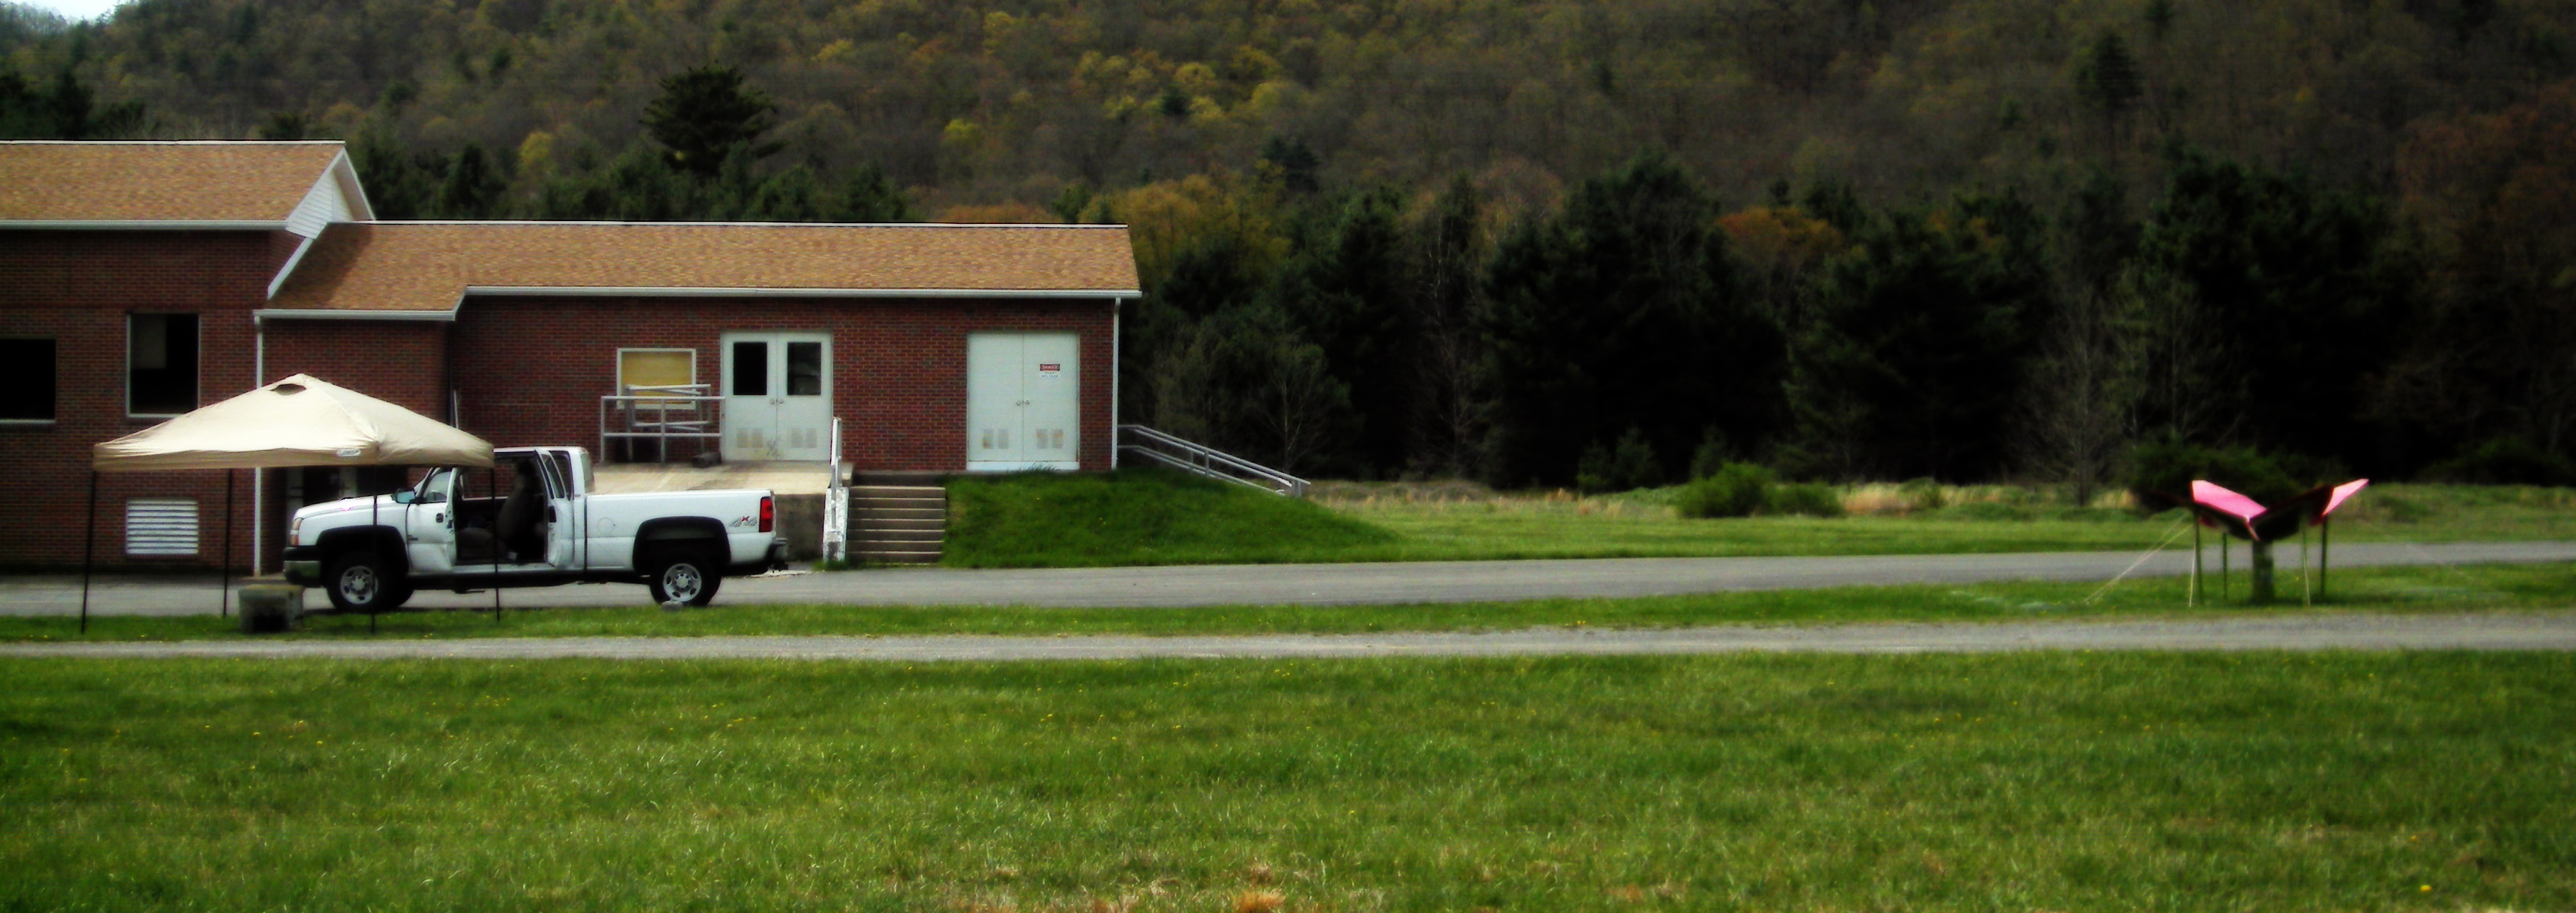
\includegraphics[width=0.95\linewidth]{SCIHI_system/figures/SCIHI_gbt_sys.jpg}
\caption{SCI-HI system with HIbiscus antenna set up on site at Green Bank in May 2013.}
\label{Fig:sys_gbt}

\end{center}
\end{figure}

%\end{minipage}%
%\begin{minipage}[b]{0.02\textwidth}
%\hspace{1cm}
%\end{minipage}%
%\begin{minipage}[b]{0.47\textwidth}
%\centering

\begin{figure}[htb]
\begin{center}
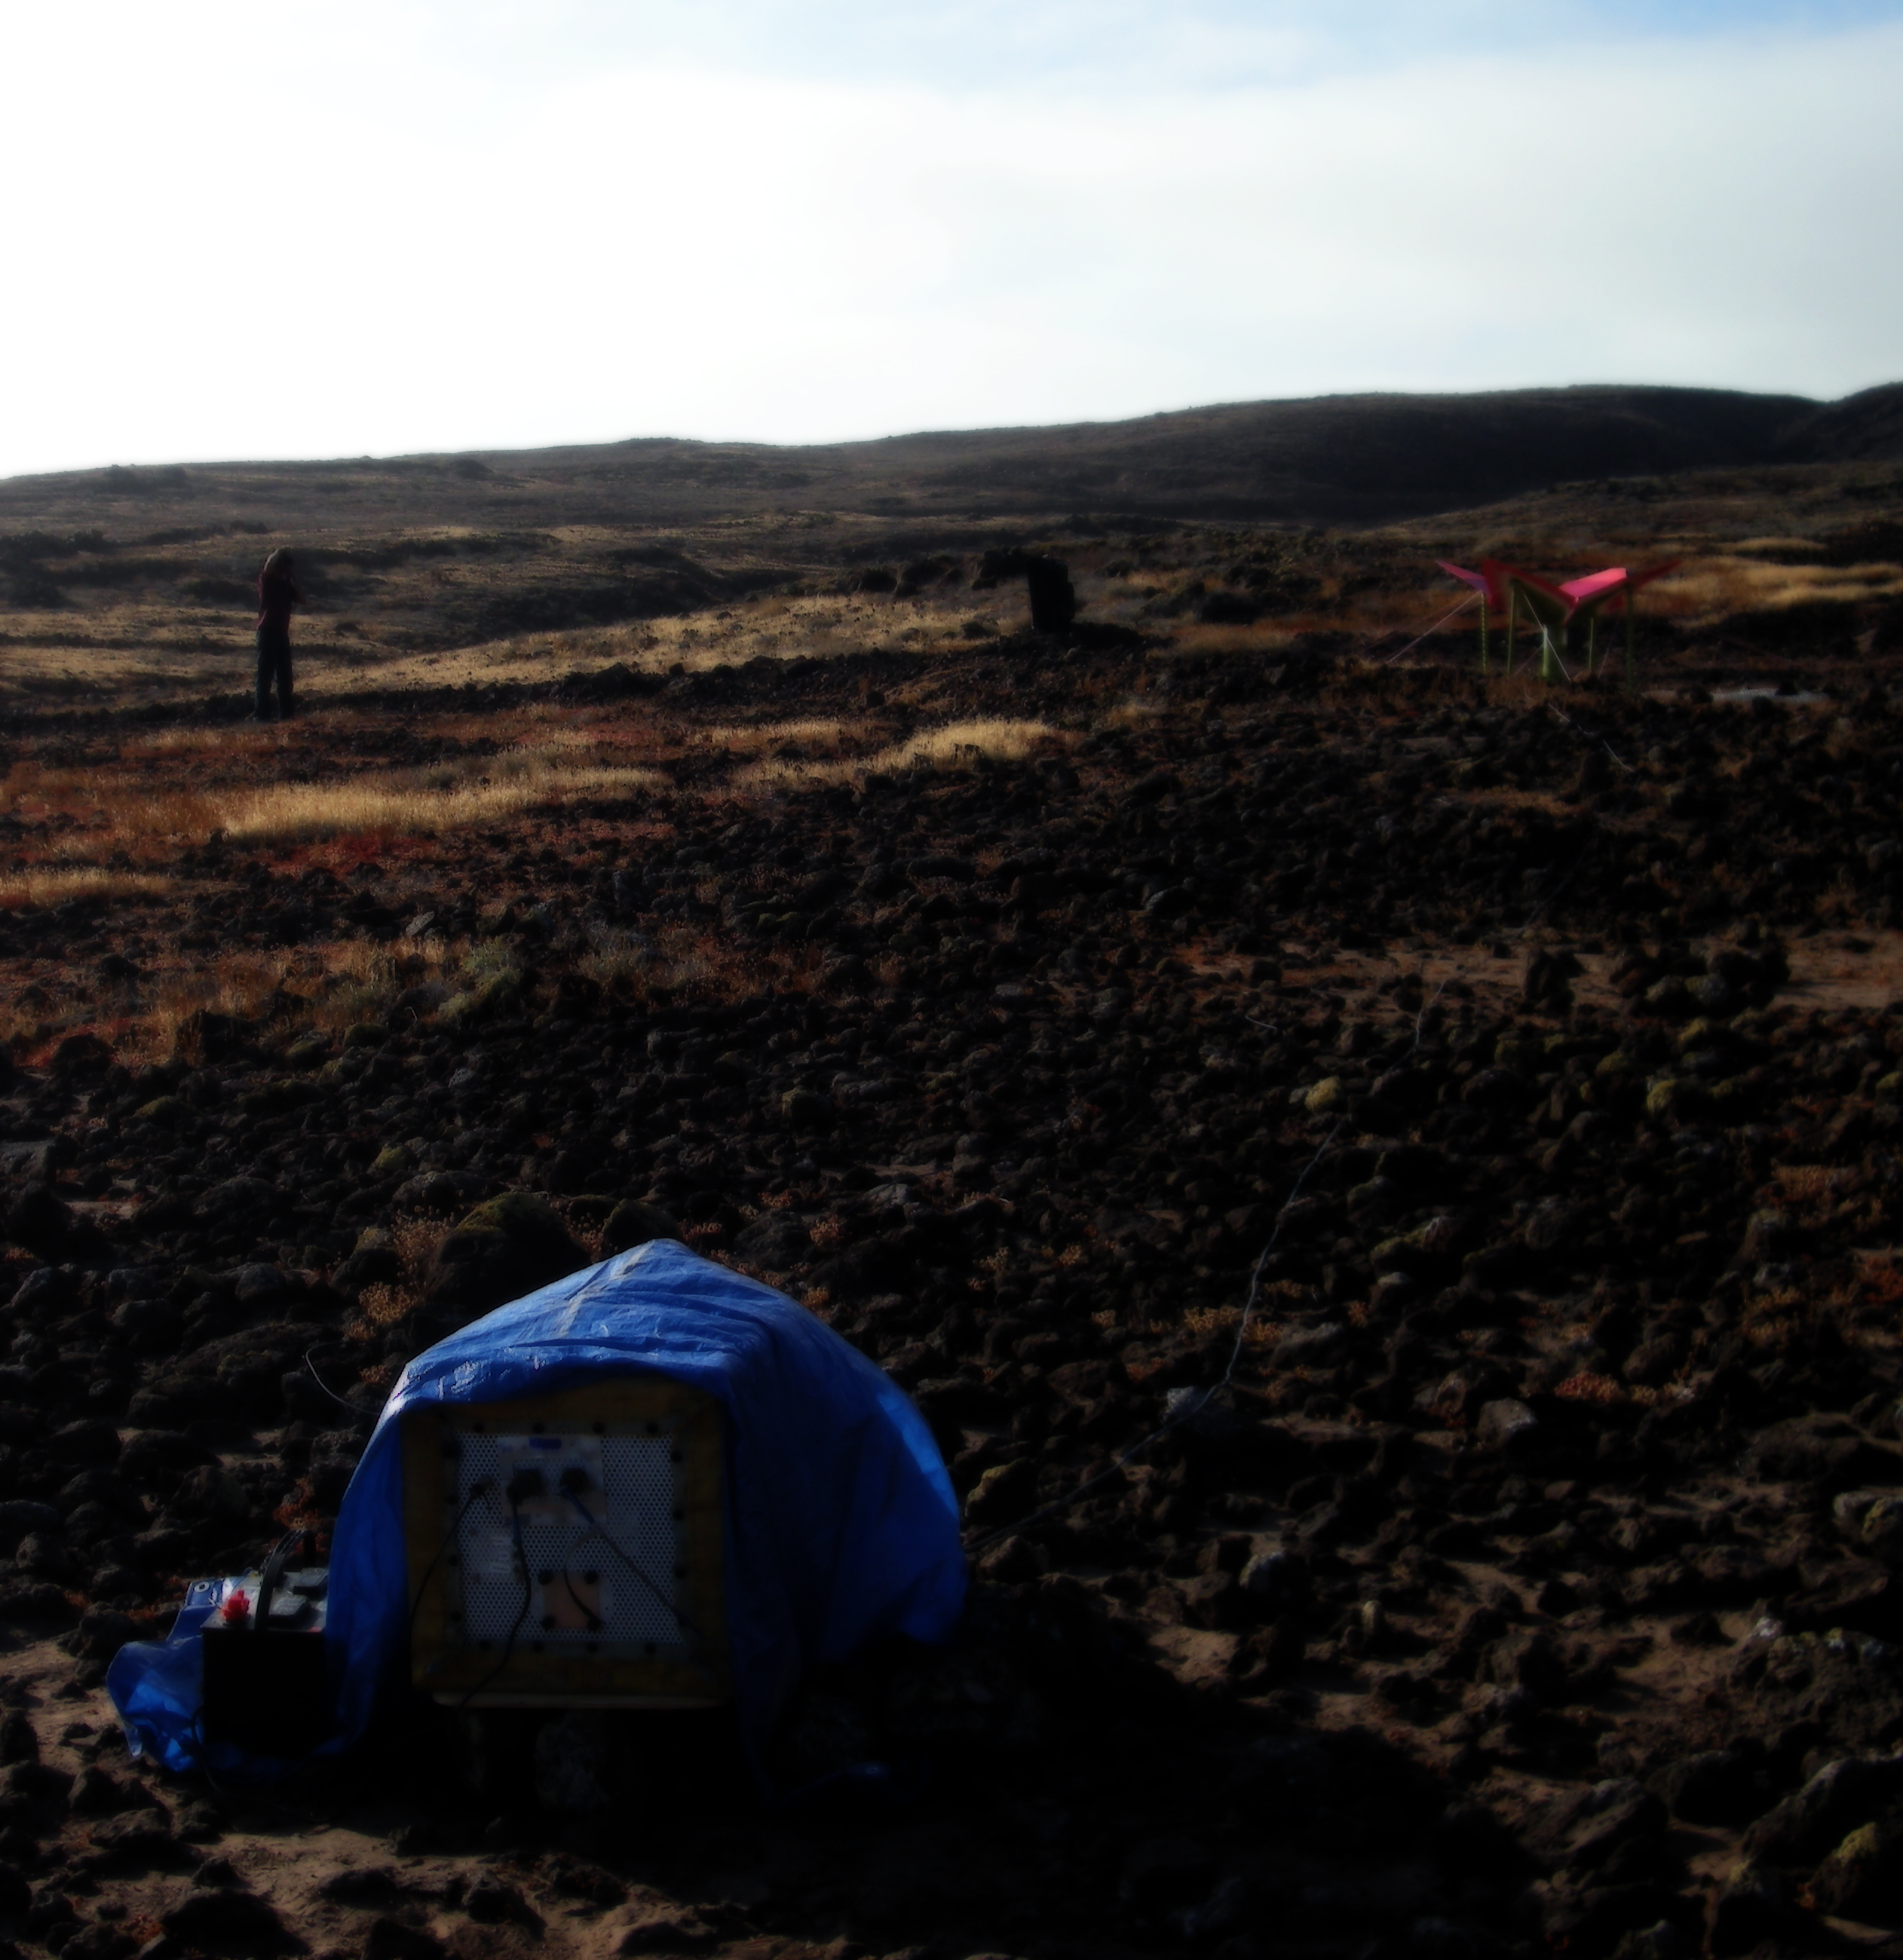
\includegraphics[width=0.85\linewidth]{SCIHI_system/figures/SCIHI_guad_sys.jpg}
\caption{SCI-HI system with HIbiscus antenna set up on site at Isla Guadalupe in June 2013}
\label{Fig:sys_guad}
%\end{minipage}

\end{center}
\end{figure}


\section{RF Electronics}

Once the signal from the sky has been collected by the antenna, it has to be transmitted to the data proccessing system in a form that the system is capable of processing. Transmission happens along a chain of radio frequency (RF) electronics. 

\textcolor{red}{Add a second level RF chain flow chart here.}
\subsection{RF Chain Overview}
For the SCI-HI system, the RF chain components are a switch, amplifiers, high and low pass filters, attenuators and a power splitter (along with the attendant cabling). Each of these components serves a specific purpose in the system. 

We can divide the RF chain into two sections based upon physical location. The first section is the antenna electronics, which sit as close to the antenna terminal as physically possible. The second section is the Faraday cage electronics, which sit next to the data processing system within a Faraday Cage. Between the two sections is a long signal cable ($\sim50-100 m$), allowing the antenna and data processing system to be placed far enough apart that the transmission of self-generated noise from the data processor is minimized (see Figures \ref{Fig:sys_gbt} and \ref{Fig:sys_guad}).

\begin{figure}[htb]
\centering
\begin{minipage}[b]{0.47\textwidth}
\centering
\includegraphics[width=0.95\linewidth]{SCIHI_system/figures/trombone_sys_switch.jpg}
\caption{Trombone antenna setup with calibration switch mounted directly below the antenna.}
\label{Fig:trombone_switch}
\end{minipage}%
\begin{minipage}[b]{0.02\textwidth}
\hspace{1cm}
\end{minipage}%
\begin{minipage}[b]{0.47\textwidth}
\centering
\includegraphics[width=0.95\linewidth]{SCIHI_system/figures/SCIHI_rf_ant_lower.jpg}
\caption{RF electronics box at the base of the trombone antenna with second stage amplifier and filters.}
\label{Fig:trombone_base}
\end{minipage}
\end{figure}

\textcolor{red}{Add a third level RF chain flow chart of just the antenna electronics here.}

\subsection{Antenna Electronics}
The antenna electronics are a calibration switch with known signal sources on some of the terminalsand two stages of amplification. In some versions of the electronics system, at least one of the RF filters was placed at the antenna end of the system but we'll discuss that component in the Faraday Cage electronics section. 

\subsubsection{Calibration Switch}
Because the SCI-HI system has a single antenna with a relatively large beam ($\sim 55^\circ$), calibrating the data from the antenna can be difficult. One way to do this calibration is to use noise source of known temperature whose signal is sent through the same RF chain as the antenna data (see Chapter \ref{Ch:Data}). 

In order to facilitate this calibration, a switch was placed at the terminal of the antenna. By making the antenna one of the inputs of the switch and matching one or more known temperature sources to the other switch inputs, data can be collected for all inputs with the same RF chain. 

We used a 6 input electromechanical switch (\textcolor{red}{Add part numbers here}) for the system. One input to the switch was connected directly to the antenna (see Figures \ref{Fig:trombone_switch} and \ref{Fig:rf_ant_mount}). The other inputs were a short terminator, a $50 \Omega$ load terminatore, a $100 \Omega$ load terminator, and an artificial noise source of known power. One input was left open. 

Switching between inputs is controlled through a cable from the Faraday Cage that carries both the power for the antenna electronics and the control signal. In addtion, the artificial noise source is turned off when that input is not enabled (to avoid noise bleeding into the antenna). We also built a manual switch control box that can be hooked up to the switch for testing. 

\begin{figure}[htb]
\centering
\begin{minipage}[b]{0.47\textwidth}
\centering
\includegraphics[width=0.95\linewidth]{SCIHI_system/figures/SCIHI_rf_ant_box.jpg}
\caption{New lucite box containing all the antenna RF electronics.}
\label{Fig:rf_ant_box}
\end{minipage}%
\begin{minipage}[b]{0.02\textwidth}
\hspace{1cm}
\end{minipage}%
\begin{minipage}[b]{0.47\textwidth}
\centering
\includegraphics[width=0.95\linewidth]{SCIHI_system/figures/SCIHI_rf_ant_box_mount.jpg}
\caption{RF electronics box attached to one of the HIbiscus antenna center mounts.}
\label{Fig:rf_ant_mount}
\end{minipage}
\end{figure}

\subsubsection{Amplifiers}
Immediatelly following the switch in the RF chain is the first stage amplifier. 

\textcolor{red}{Add general discussion of S-parameters and Transmission Efficiency followed by a section on the different types of amplifiers that we tried and why we selected the one that we did. This should include a figure showing the amplifier S11 signals.}

\paragraph{S-parameters}

\paragraph{Transmission Efficiency}

\paragraph{Amplifier Selection}

\paragraph{Multi-stage Amplification}
Because the $\sim50-100 m$ signal cable will attenuate signals travelling down its length, a second stage amplifier was added to the system to increase the gain of the signal. Both amplifiers use DC power supplied by the same power cable as the switch. Because different levels of DC power were needed for the varying electronic components, voltage regulation circuits were also included in the antenna electronics housing. 

To maintain transmission efficiency, the first and second stage amplifiers' impedence had to match well. This was accomplished by using the same amplifier type for both stages. Initially the second stage amplifier was placed at the base of antenna (see Figure \ref{Fig:trombone_base}). However, this placement resulted in reflections in the signal whose period corresponded to the cable length between the two amplifiers. \textcolor{red}{May try to make a plot that shows this.} Therefore, the second stage amplifier was moved to a position immediately following the first stage amplifier (see Figure \ref{Fig:rf_ant_box}), which removed the effect. The total gain of the amplifiers was $\sim$50 dB over the entire frequency band. 

\textcolor{red}{Add a third level RF chain flow chart of just the Faraday cage electronics here.}

\subsection{Faraday Cage Electronics}
Once the signal has travelled down a long cable from the antenna, there are a few electronic stages that it must pass through prior to entering the data processing system. A third stage amplifier is needed to compensate for the attenuation caused by the long cable, filters are needed to keep signals from outside the frequency band of interest from overloading the data processing system, and a signals splitter used to achieve the necessary data sampling rate. All of these electronics, as well as the data processing system, were placed inside a Faraday cage designed specifically to accomodate them. 

\begin{figure}[htb]
\centering
\begin{minipage}[b]{0.36\textwidth}
\centering
\includegraphics[width=0.95\linewidth]{SCIHI_system/figures/SCIHI_fcage_old.jpg}
\caption{Faraday cage around data processing system as setup in October 2012.}
\label{Fig:fcage_old}
\end{minipage}%
\begin{minipage}[b]{0.02\textwidth}
\hspace{1cm}
\end{minipage}%
\begin{minipage}[b]{0.58\textwidth}
\centering
\includegraphics[width=0.95\linewidth]{SCIHI_system/figures/SCIHI_filter.jpg}
\caption{System power and control signal filter box for one of the Faraday Cages.}
\label{Fig:fcage_filter}
\end{minipage}
\end{figure}

\subsubsection{Faraday Cage Design}
The design of the Faraday Cage for the SCI-HI system was inspired by the dual requirements of space and portability. Because the wavelengths being studied with the system are $\geq 2$ meters, metal mesh could be used in place of solid metal for the sides of the cage. This mesh is considerably lighter than solid metal, but does not hold its structure. So I came up with a design that uses a metal mesh bag with a PVC pipe framework placed inside to hold its shape (see Figure \ref{Fig:fcage_old}). The mesh bag folds up like a paper bag and the PVC framework can be disassembled, allowing it to be packed up into a suitcase. 

Access to the Faraday cage was supplied through the front panel, which attached to the rest of the bag through a set of metal snaps spaced less than 20 cm apart. This front panel included access ports for the signal cable, as well as the power and switch control cable. Multiple versions of the Faraday cage were constructed, but all of them used the same mesh bag system (see Figures \ref{Fig:fcage_int} and \ref{Fig:fcage_new}). 

\begin{figure}[htb]
\centering
\begin{minipage}[b]{0.44\textwidth}
\centering
\includegraphics[width=0.95\linewidth]{SCIHI_system/figures/SCIHI_fcage_int.jpg}
\caption{Faraday cage around data processing system as setup in June 2013.}
\label{Fig:fcage_int}
\end{minipage}%
\begin{minipage}[b]{0.02\textwidth}
\hspace{1cm}
\end{minipage}%
\begin{minipage}[b]{0.50\textwidth}
\centering
\includegraphics[width=0.95\linewidth]{SCIHI_system/figures/SCIHI_fcage_new.jpg}
\caption{Faraday Cage with double shielding around data processing system, currently under development.}
\label{Fig:fcage_new}
\end{minipage}
\end{figure}

\subsubsection{Power Filters}
Because the power and switch control cable carried DC power out to the antenna electronics, it needed to be filtered to keep RF signals from using the cable to escape the Faraday Cage. To accomplish this, a set of filter boxes were placed in the DC power and switch control signal lines. These filter boxes (see Figure \ref{Fig:fcage_filter}) were low pass filters with over 40 dB of attenuation at 40 MHz. Two stages of filtering were included to ensure that there was no signal transmission through the DC power lines. 

Once the battery was placed outside of the Faraday Cage, filters also had to be used between the battery and the electronics inside the cage. The same filters used for the DC power and switch control cable were also used to make sure that RF signals didn't use the power supply cable from the battery to transmit outside the Faraday Cage.  


\subsubsection{System Power} \label{Sec:sys_power}
The entire system was powered using deep-cycle automotive batteries. These batteries supplied 12 V unregulated power, which was used by both the data processing system and the RF electronics. Initial designs of the Faraday cage had the DC battery stored inside the Faraday Cage, as shown in Figure \ref{Fig:fcage_old}. Later, the battery was moved outside the cage for easier access (see Figure \ref{Fig:fcage_int}). A fully charged battery could power the entire system for $\sim$12-15 hours. 

Charging batteries was a big part of the support process for the SCI-HI system. Keeping the system running continually required at least 3 batteries with regular access to a battery charger and transport between the SCI-HI site and the battery charging location 2-3 times a day. 

An alternative to running off batteries is to use a small portable gasoline or diesel generator. Using this generator would cut down on the number of site visits required, as the generator would run constantly with only occasional stops to top off the fuel. However, using a generator also provides a new source of RF noise (particularly a gasoline generator with spark plugs). Placing the generator inside its own Faraday Cage should attenuate this noise, but it is a factor that must be accounted for in selecting a power source. 

\subsubsection{RF Filters and Amplification}
Once the signal from the antenna entered the Faraday Cage, the first part of the RF chain was a set of filters. These filters were a low pass filter at 200 MHz (\textcolor{red}{add part number here}) and a high pass filter at 30 MHz (\textcolor{red}{add part number here}). The low pass filter was placed to prevent signals from higher frequencies ($\geq 200$ MHz) from aliasing into the frequency range where we were observing. The high pass filter was placed to prevent signals from the AM band and below overloading the sampling system, which could affect the overall system gain or create spurious signals in the observing band. 

After the signal has passed through the long cable and the filters, it is necessary to add another level of amplification to the system. This final stage of amplification is to bring the signal levels to a point where they can be clearly distinguished from system noise by the data processing system and adds $\sim25$ dB of gain. The amplifier used here is a \textcolor{red}{Add part number here} minicircuits amplifier, which is supplied with regulated power from the DC source. 

\subsubsection{RF Signal Splitting} \label{Sec:hard_split}
The analog to digital conversion (ADC) card used in the data processing system is limited to a 250 MSamples-per-sec sampling rate, but the bandwidth of the system is over 125 MHz. In order to expand the operating range of the ADC, a hardware $''$trick$''$ is used.

The signal from the antenna is split into two identical signals with a \textcolor{red}{Add part number here} splitter. Both signals are then sent to the ADC using two of the input ports. However, the lengths of the cables placed between the two outputs of the splitter and the two input ports of the ADC are slightly different. The difference (\textcolor{red}{Add exact length here} is exactly matched such that a sample taken from one input port is has been delayed by 2 ns compared to the other input port. If the signals from both ports are combined, the data now appears to have been sampled at 500 MSamples-per-sec. 


\section{Data Processing System}

\subsection{Data Processing Pathway}
As discussed in Section \ref{Sec:hard_split}, signals from the sky enter the system via two ports of an analog to digital conversion (ADC) card. For the SCI-HI system, we used a \textcolor{red}{add part name and number here} card. Data is collected for one second of integration, with the interleaving stragegy producing 500 MSamples of data. 

Storing the entire dataset for each second would require a great deal of space. Instead, a fast fourier transform (FFT) is performed on the dataset. The frequency spectrum produced by the FFT takes up much less space (\textcolor{red}{How much less?}) and is stored by the system. The process is then repeated for another second of data. 

Because of the design of the system, collecting new data can only be done after the FFT is complete. This means that the system is less than 100\% efficient, or it takes longer than 1 second to record the frequency spectrum of 1 second of data. Initially the FFT calculation was quite time consuming ($\sim 30-60$ seconds), but improvements to the software and hardware have decreased this calculation rate to $\sim 2$ seconds. This means that the system has a maximum duty cycle of $\sim30$\%. 

All of the frequency spectrum data is stored locally on the hard drive of the processing system. The relatively small data volume ($\sim 2$ Gb per day) means that data transfer can be done using small USB drives. During deployment, data was removed from the hard drive 2-3 times a day and stored locally on multiple laptop computers and external hard drives before being uploaded to a server upon return to $''$civilization$''$ (aka the lab). 

\subsection{System Control and User Interface}
In addition to the data processing software, a graphical user interface was designed for diagnostic and control purposes. This interface displays the most recent frequency spectrum collected by the system and lets the user set the current data collection mode (including switch control). The user can choose to either take a single data set with any of the switch positions (Antenna, 50 $\Omega$, Short, Noise Source, 100 $\Omega$), or take continual data with a set number of Antenna datasets followed by a single dataset from each of the calibration sources. \textcolor{red}{Add screenshot of the UI here}

The system default upon start-up is to run in continual data collection mode with the number of antenna iterations as set by the system when it was previously used. To lower the power consumption and space requirements of the system, it is designed to be run without a monitor, mouse and keyboard. Instead, the system can be controlled by an external system through an ethernet port. This port is only used when the system needs to be checked.

\subsection{Control Computer}
The data processing system can be diagnosed using a personal computer (such as a laptop) with an ethernet port. However, an additional diagnostic computer was also developed for the SCI-HI system. This computer is a Raspberry Pi\footnote{www.raspberrypi.org} with a small monitor, mouse and ethernet port. \textcolor{red}{Add picture of the diagnostic computer.} Using this small computer, we can quickly check that the system is working properly and run simple diagnostics.

\subsection{Power Supply and Consumption}
In order to power the data processing system, a computer power supply had to be selected that matched the system power source (DC battery). Initially, we started with a typical AC computer power supply and a DC to AC inverter that converted the incoming DC power from the batteries into AC power that the computer could handle. 

While using an inverter is the simplest solution, it is very energy inefficient.  \textcolor{red}{Add exact inefficiency of the inverter we were using in percentages.} Additionally, any failure of the inverter can crash the entire system. Therefore, we decided to switch to an entirely DC system by replacing the AC power supply for the computer with a power supply that takes input DC power. \textcolor{red}{Add original DC power supply part number here.} 

Utilizing this power supply greatly lowered our power consumption. However, we found that the power supply we selected was not reliable. Most of the DC power supplies on the market are designed for automotive applications, where they are only needed for short durations rather than continual use. In particular, the DC power supply was particularly unhappy when running in a low battery situation. We are currently exploring different alternatives, as discussed in Section \ref{Sec:sys_power}. 

\begin{figure}[htb]
\centering
\begin{minipage}[b]{0.52\textwidth}
\centering
\includegraphics[width=0.95\linewidth]{SCIHI_system/figures/SCIHI_comp.jpg}
\caption{Current version of the data processing system assembled inside a Faraday Cage box.}
\label{Fig:new_comp}
\end{minipage}%
\begin{minipage}[b]{0.02\textwidth}
\hspace{1cm}
\end{minipage}%
\begin{minipage}[b]{0.42\textwidth}
\centering
\includegraphics[width=0.95\linewidth]{SCIHI_system/figures/SCIHI_water_cooling_pipe.jpg}
\caption{Part of the water cooling system for the data processing machine.}
\label{Fig:water_pipe}
\end{minipage}
\end{figure}

\subsection{System Noise Generation}
Deployment to Isla Guadalupe in June 2013 indicated that our Faraday Cage design had insufficient attenuation of self-generated RFI from the data processing system. This problem was not identified until deployment at the site due to the low levels of RFI compared to external RFI at the testing locations. Self-generated RFI was particularly noticeable above 90 MHz, (see Figure \textcolor{red}{Add time average plot here})but may be present in the data in the lower frequencies as well. Our data indicated that the strength of the self-generated RFI was correlated with the voltage (or charge level) of the DC batteries (see Figure \textcolor{red}{Add waterfall plot here.}). 

In order to address this problem, a more robust Faraday Cage was designed for the SCI-HI system. This Faraday Cage is a double layer cage (see Figure \ref{Fig:new_comp}) with the data processing system placed inside a solid aluminum sealed box and a second Faraday cage with the rest of the electronics placed around the inner box. 

Using a set of two walkie talkies, the aluminum box was tested to show attenuation $\geq$70 dB before modification. This was measured by placing one walkie talkie inside the box in recieve mode and transmitting a signal with the other walkie talkie. If the attenuation was smaller than the transmitted signal, then the recieving signal would make a noise. Even transmitting from less than 1 meter from the box, the signal was not picked up by the reciever. 

However, the problem with using a solid metal Faraday Cage is that it becomes very difficult to cool the system. we designed a water cooling system using copper tubing mounted to the inside of the box (see Figure \ref{Fig:water_pipe}) and heat fins mounted to the outside of the box. A fan with its own Faraday cage was also mounted to the outside of the box to aid heat transfer. This system has been found sufficient for cooling in lab tests, but has not yet been tested in the field. 

\section{Summary}

The SCI-HI system has been developed to meet the constraints set in Section \ref{Sec:sysover} and features the optimized HIbiscus antenna, a compact RF electronic chain, and a robust, low-power data processing system. 
